%----------------------------------------------------------------------------------------
%	PACKAGES AND OTHER DOCUMENT CONFIGURATIONS
%----------------------------------------------------------------------------------------

\documentclass{article} % paper and 12pt font size
\usepackage{amsmath,amsfonts,amsthm} % Math packages
\usepackage[margin=1in]{geometry}
\usepackage[ruled,vlined]{algorithm2e}
\usepackage{graphicx}
\usepackage{float}
\usepackage[parfill]{parskip}
\usepackage[labelsep=quad,indention=10pt]{subfig}
\setlength{\paperwidth}{8.5in}
\setlength{\paperheight}{11in}

%----------------------------------------------------------------------------------------
%	TITLE SECTION
%----------------------------------------------------------------------------------------

\newcommand{\horrule}[1]{\rule{\linewidth}{#1}} % Create horizontal rule command with 1 argument of height

\title{	
\normalfont \normalsize 
\textsc{University of Texas at Austin, CS 391L} \\
\horrule{0.6pt} \\[0.4cm] % Thin top horizontal rule
\huge Homework 1 - Eigendigits \\[0.4cm]
\large Write Up  \\
\horrule{2pt} \\[0.5cm] % Thick bottom horizontal rule
}
\author{Venketaram Ramachandran\\
vr7948 - venket@cs.utexas.edu} % Your name
\date{\normalsize\today} % Today's date or a custom date

\begin{document}

\maketitle % Print the title

%----------------
% Approach
%----------------
\section{Overview}

In this assignment, I utilized Principle Component Analysis to help classify images of digits. The images, themselves, were provided as 8bit, single-channel grayscale images (i.e. each value for a pixel varies from 0 to 255) sized 28x28 pixels each. Figure 1 shows examples of the digit image provided in the training data.

\begin{figure}[h]%
	\centering
    	\subfloat[Training example of a 9]{%
        	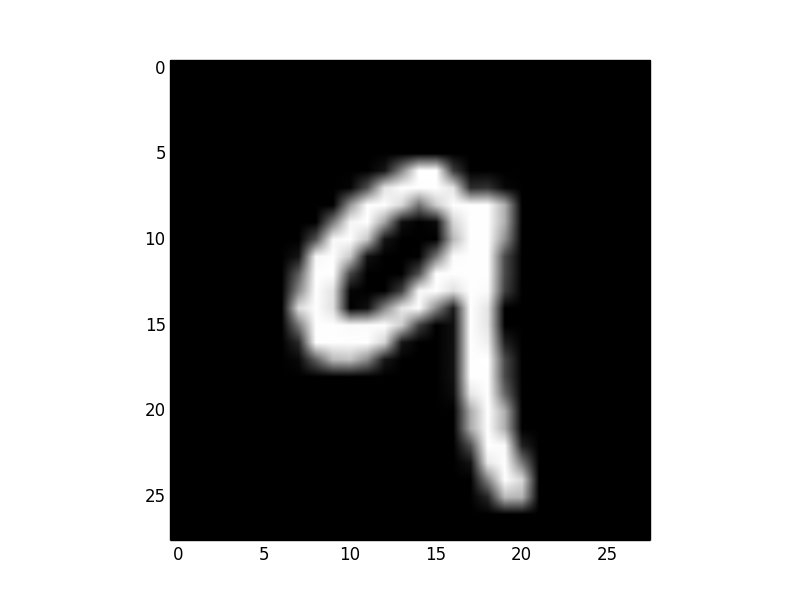
\includegraphics[width=70mm]{figure_1.png}%
            \label{fig:left}%
        }\hfill%
        \subfloat[Training example of a 0]{%
        	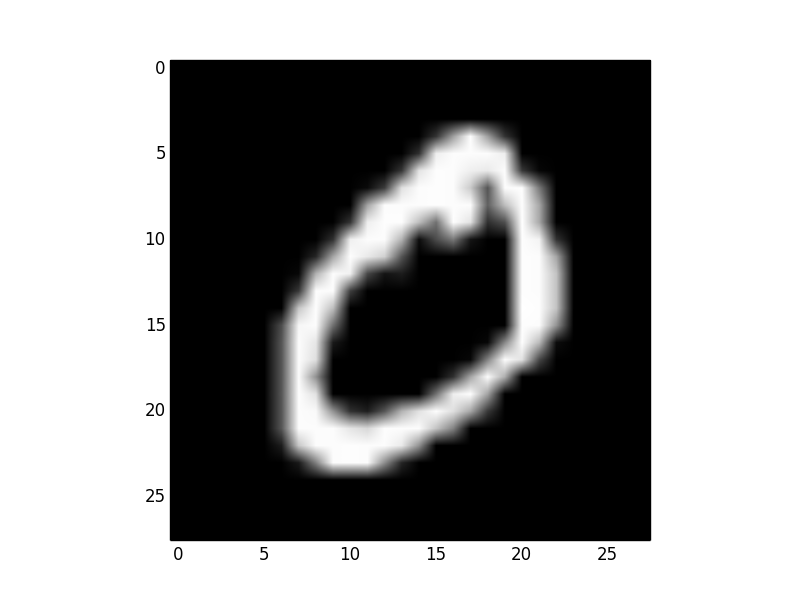
\includegraphics[width=70mm]{second_training_example.png}%
            \label{fig:right}%
        }
    \caption{\textit{Two training examples of digits from the digits.mat file}}
    \label{fig:default}
\end{figure}

The premise of the experiments in the assignment involved attempting to utilize Principal Component Analysis to analyze the digit images based on the images' principal components (e.g. the features contributing the most variance). In doing so, Principal Component Analysis offers the possibility of dimensionality reduction when analyzing the image data. In general, the number of features extracted can significantly outnumber the number of training examples available. As such, Principal Component Analysis' offer of dimensionality reduction can help greatly in training and classification tasks, as the focus becomes only on the components that are the most significant. In this assignment, in particular, I retrieved the eigenvectors of the covariance matrix of the digit training examples of digits. I, then, utilized that to select the top significant eigenvectors (based on the relative largeness of their associated eigenvalue) to project the digit images to the reduced eigenspace for classification by the k-Nearest Neighbors algorithm.

\section{Implementation}

The experiments done below leveraged the Numpy, Scipy, and Scikit-learn utilities in Python to read the input matlab file, perform linear algebra operations, and perform k-Nearest Neighbors classification. The experiments themselves and the data shown below can be reproduced through the execution of a single script. Please refer to the README file in the submitted code package for further details. 

\subsection{Retrieving Eigenvectors}

The code to retrieve eigenvectors utilized the following algorithm described in Algorithm 1:

\begin{algorithm}
  \caption{\textsc {Find-Eigendigits} \label{IR2}}
  \SetKw{KwInitialize}{Initialize:}	
  \KwIn{matrix of images A where A.shape = (number of pixels,number of images)}
  \KwOut{The mean column vector of A, a matrix of eigenvectors sorted by associated eigenvalue}
  \Begin{
  	\(V\) = compute mean column vector of A \\
    \(B\)= \(A - V\) \\
    \(A_{reduced}\) = \(B^T \times{B}\) \\
    \(C\) = compute covariance matrix of \(A_{reduced}\) \\
    \(E_{small}\) = compute eigenvectors of \(C\) \\
    \(E_{large}\) = \(B \times{E_{small}}\)\\
    sort eigenvector order in \(E_{large}\) by associated eigenvalue \\
    
    \Return \(V,E\)
  }
\end{algorithm}

\subsection{Classification}

With the eigenvectors and a particular submatrix of top eigenvectors selected, I utilized the following approach described in Algorithm 2 for classification:

\begin{algorithm}
  \caption{\textsc {Classify-Digit-Images} \label{IR2}}
  \SetKw{KwInitialize}{Initialize:}	
  \KwIn{eigenmatrix of top eigenvectors \(E\), mean column vector V, neighbor size \(K\), training images \(I_{tr}\), training labels \(L_{tr}\), test images \(I_{te}\), test labels \(L_{te}\)}
  \KwOut{Classification accuracy score of test images with test labels}
  \KwInitialize{k-Nearest Neighbor classifier \(N\) with size \(K\) and using euclidean distance} \\
  \Begin{
	\(I_{tr-projected}\) = \(E^T\times((I_{tr}-V))\) \\
	\(I_{te-projected}\) = \(E^T\times((I_{te}-V))\) \\
    \(N\).train(\(I_{tr-projected}\), \(L_{tr}\)) \\
    \(classified_{correct}\) = 0 \\
  	\For{each test image \(t\) in \(I_{te-projected}\)}{
    	\(classification\) = N.classify(\(t\)) \\
    	\If{classification matches associated label in \(L_{te}\)}{
        	\(classified_{correct}\) += 1 
        }
    }
    
    \Return \(\frac{classified_{correct}}{L_{te}.size}\)
  }
\end{algorithm}

\section{Experiments and Results}

The three main variables in the experiments were:

\begin{itemize}
  \item \textbf{\(T\)} - The number of training examples chosen. 
  \item \textbf{\(E\)} - The number of top eigenvectors chosen
  \item \textbf{\(K\)} - The value chosen for k for the k-Nearest Neighbor classifier 
\end{itemize}

The remainder of this section describes the experiments done to test the significance of the three variables on the overall classifier and the classifier accuracy.

\subsection{Varying Number of Training Examples}

\subsubsection{Setup}

I ran the overall eigenvector retrieval and classification procedure for each \(\left\{ T,E,K \right\}\) combination, where \(T \in \{500,1000,1500,2000,2500,3000,3500,4000,4500,5000\}\), \(E \in \{100, 200, 300, 400, 500\}\), and \(K \in \{1,3,5,7\}\). 

I initially considered \(K\) values much greater than 10. However, I found that they performed poorer than smaller values of \(K\) for the sets of training examples I used. For the sake of brevity and performance limitations, I've omitted those values of \(K\) and instead focused on the values of \(K\) mentioned above. This point is further discussed in Section 3.3.2.

\subsubsection{Results and Observations}

Intuitively, I expected the classification accuracy to increase as the number of training examples increased. Based on my experiments, my intuition was correct, as reflected in Figure 2.

\begin{figure}[h]%
	\centering
    	\subfloat[K=1 and various E]{%
        	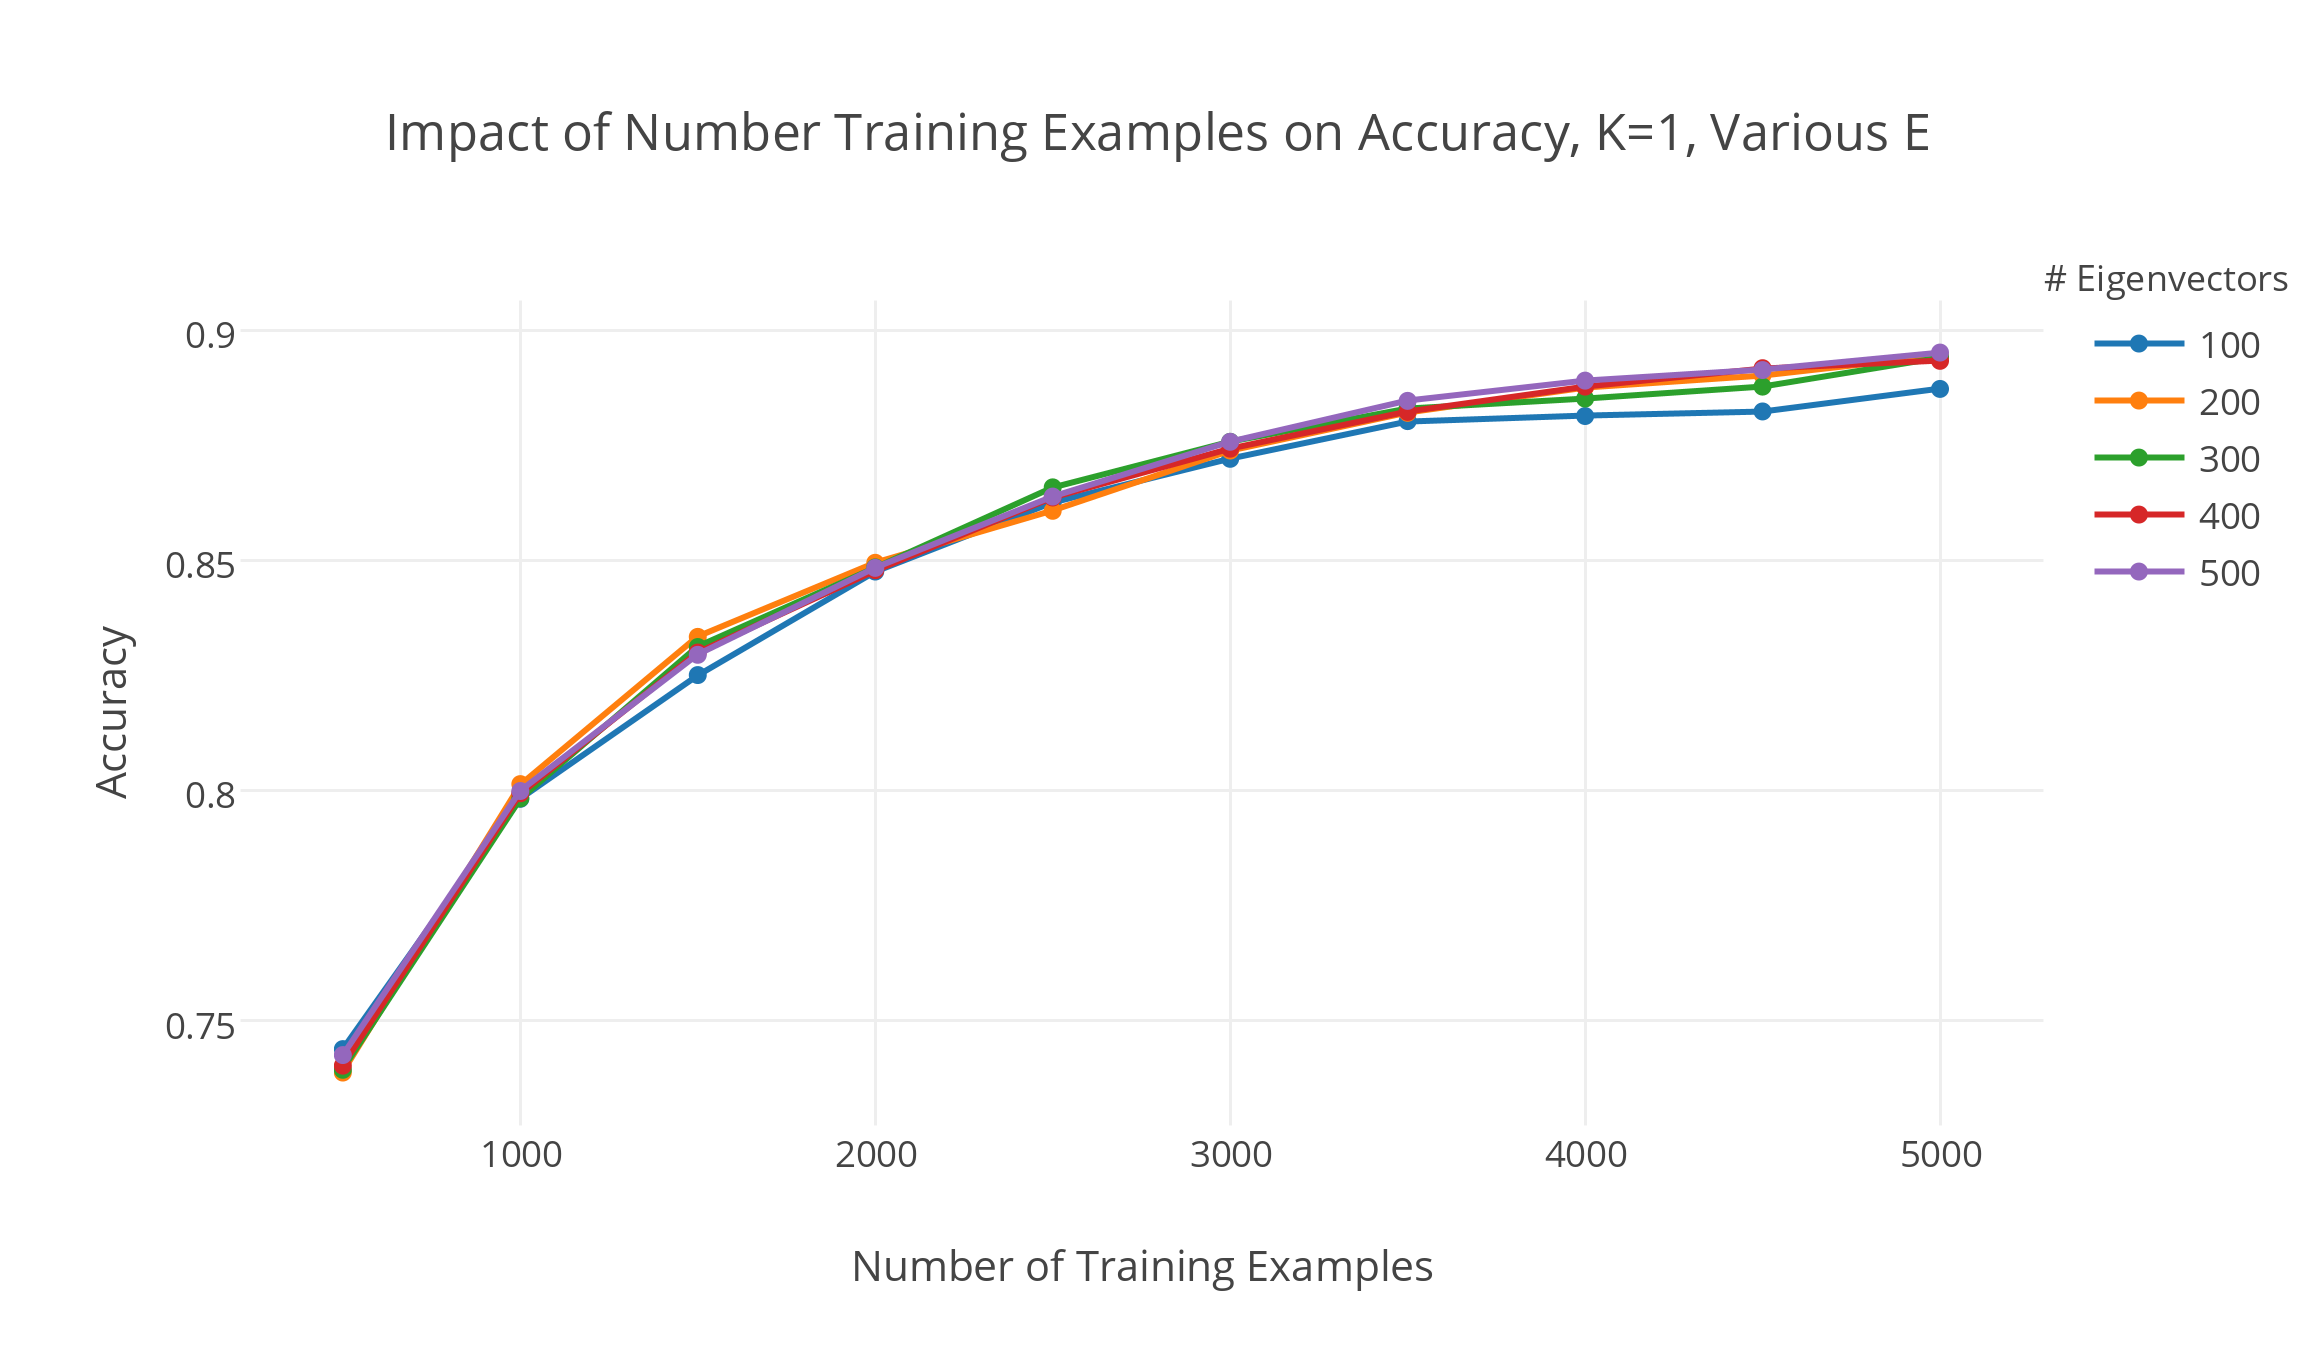
\includegraphics[width=80mm]{impact_of_number_training_examples_on_accuracy2c_k12c_various_e.png}%
            \label{fig:left}%
        }\hfill%
        \subfloat[K=3 and various E]{%
        	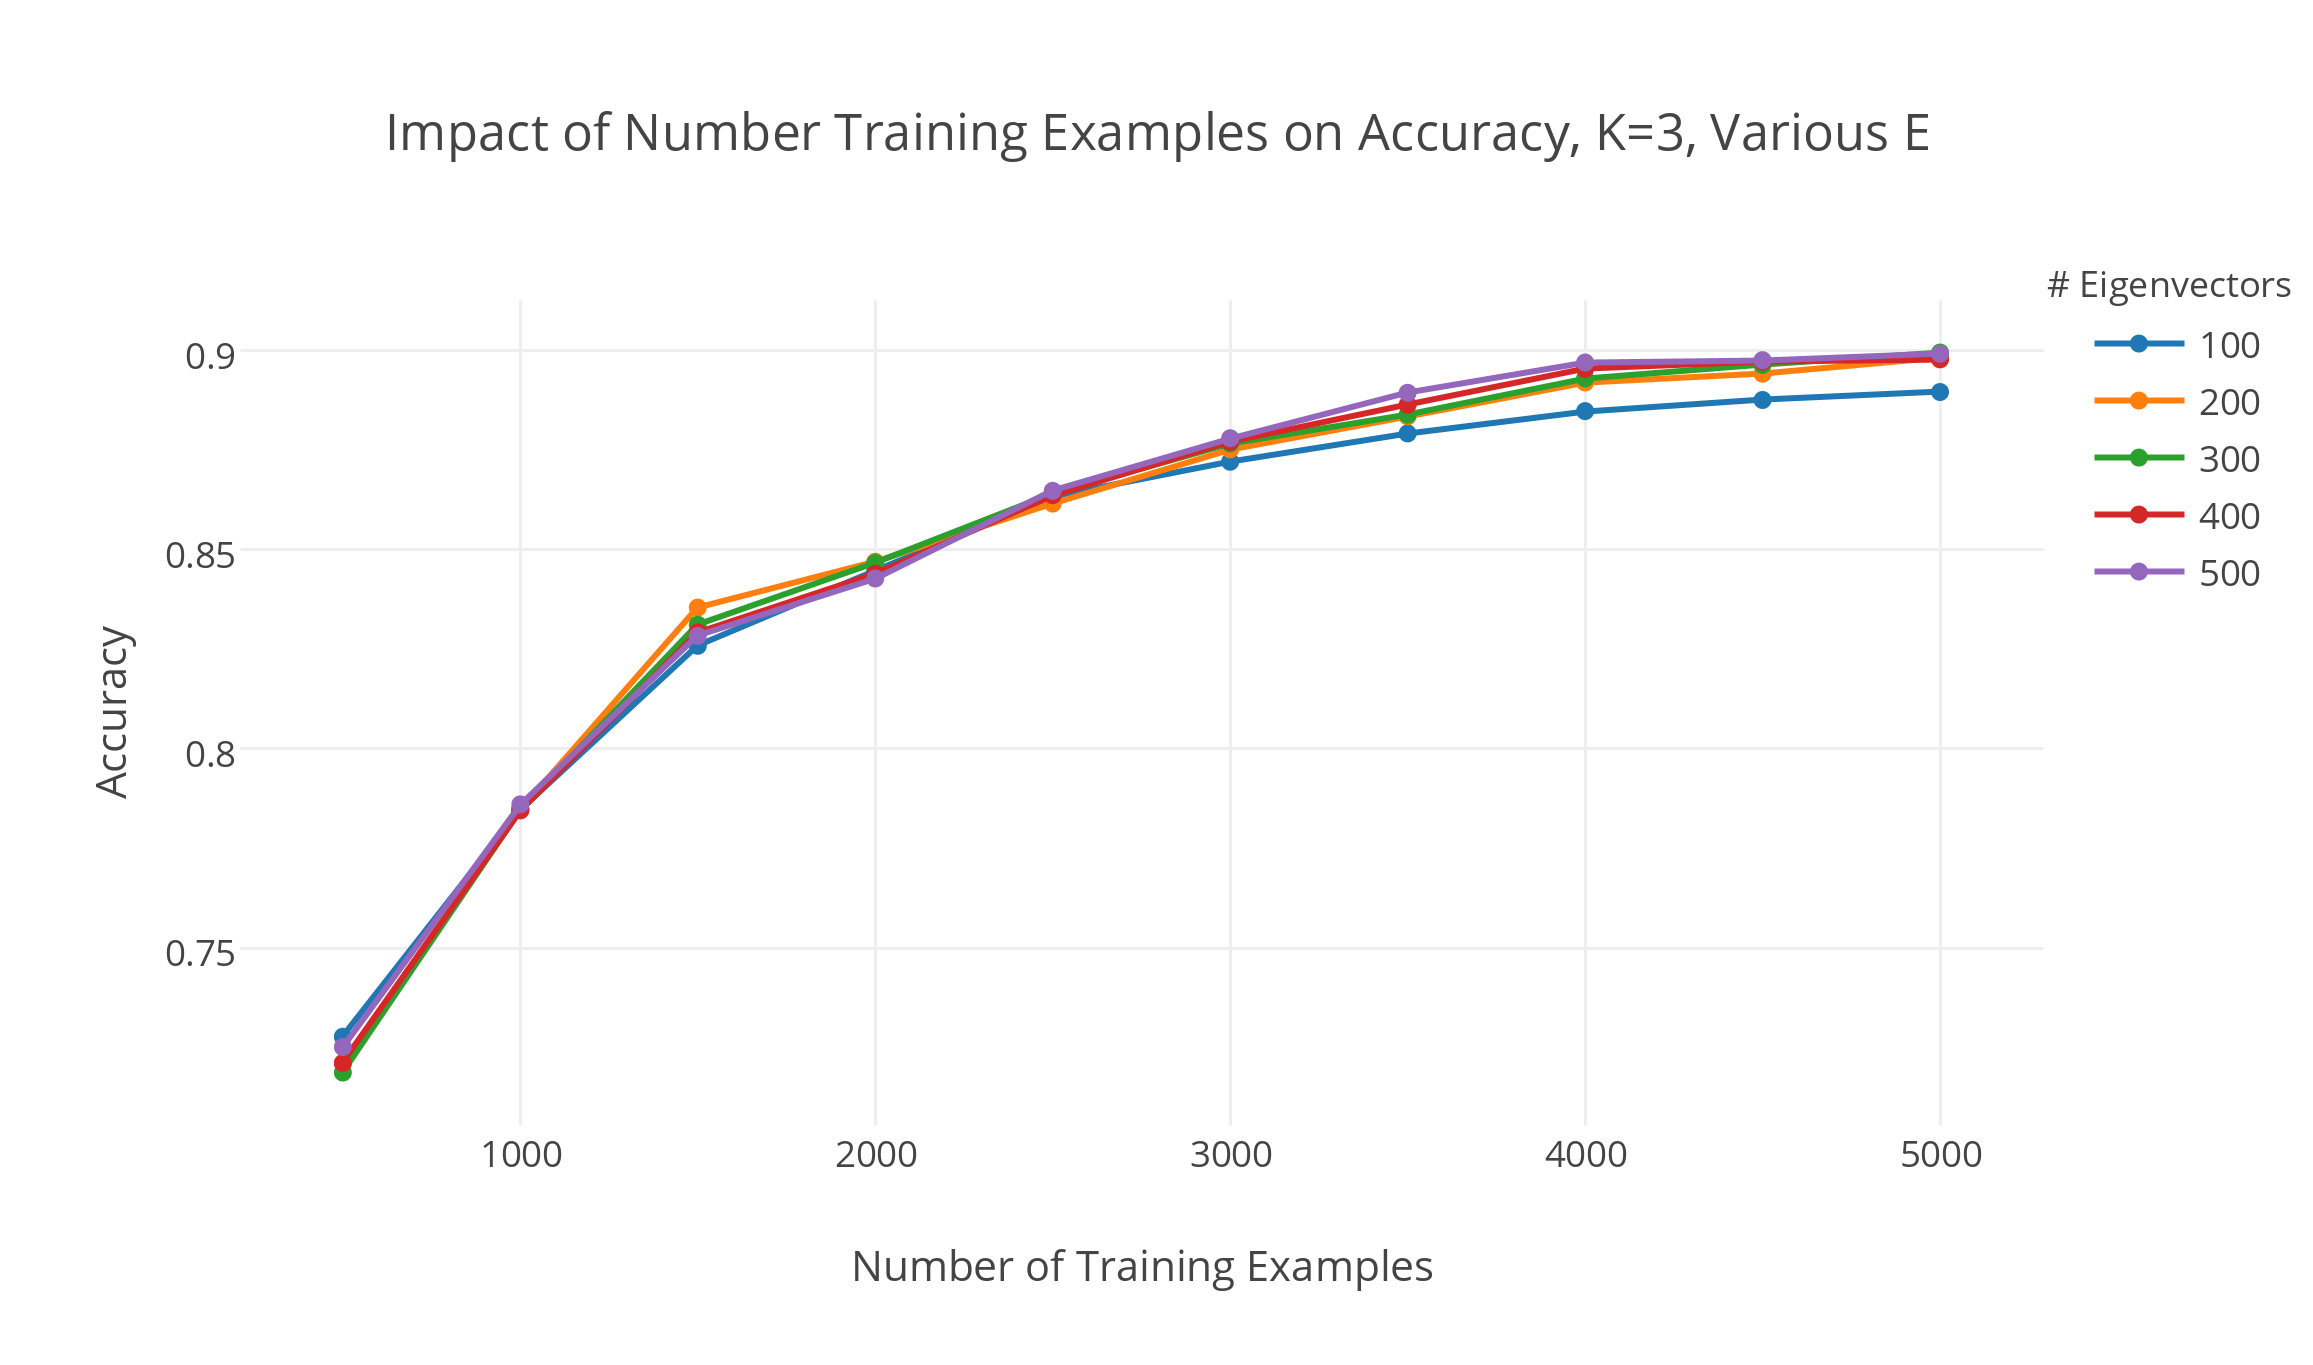
\includegraphics[width=80mm]{impact_of_number_training_examples_on_accuracy2c_k32c_various_e.png}%
            \label{fig:left}%
        }\hfill%
        \subfloat[K=5 and various E]{%
        	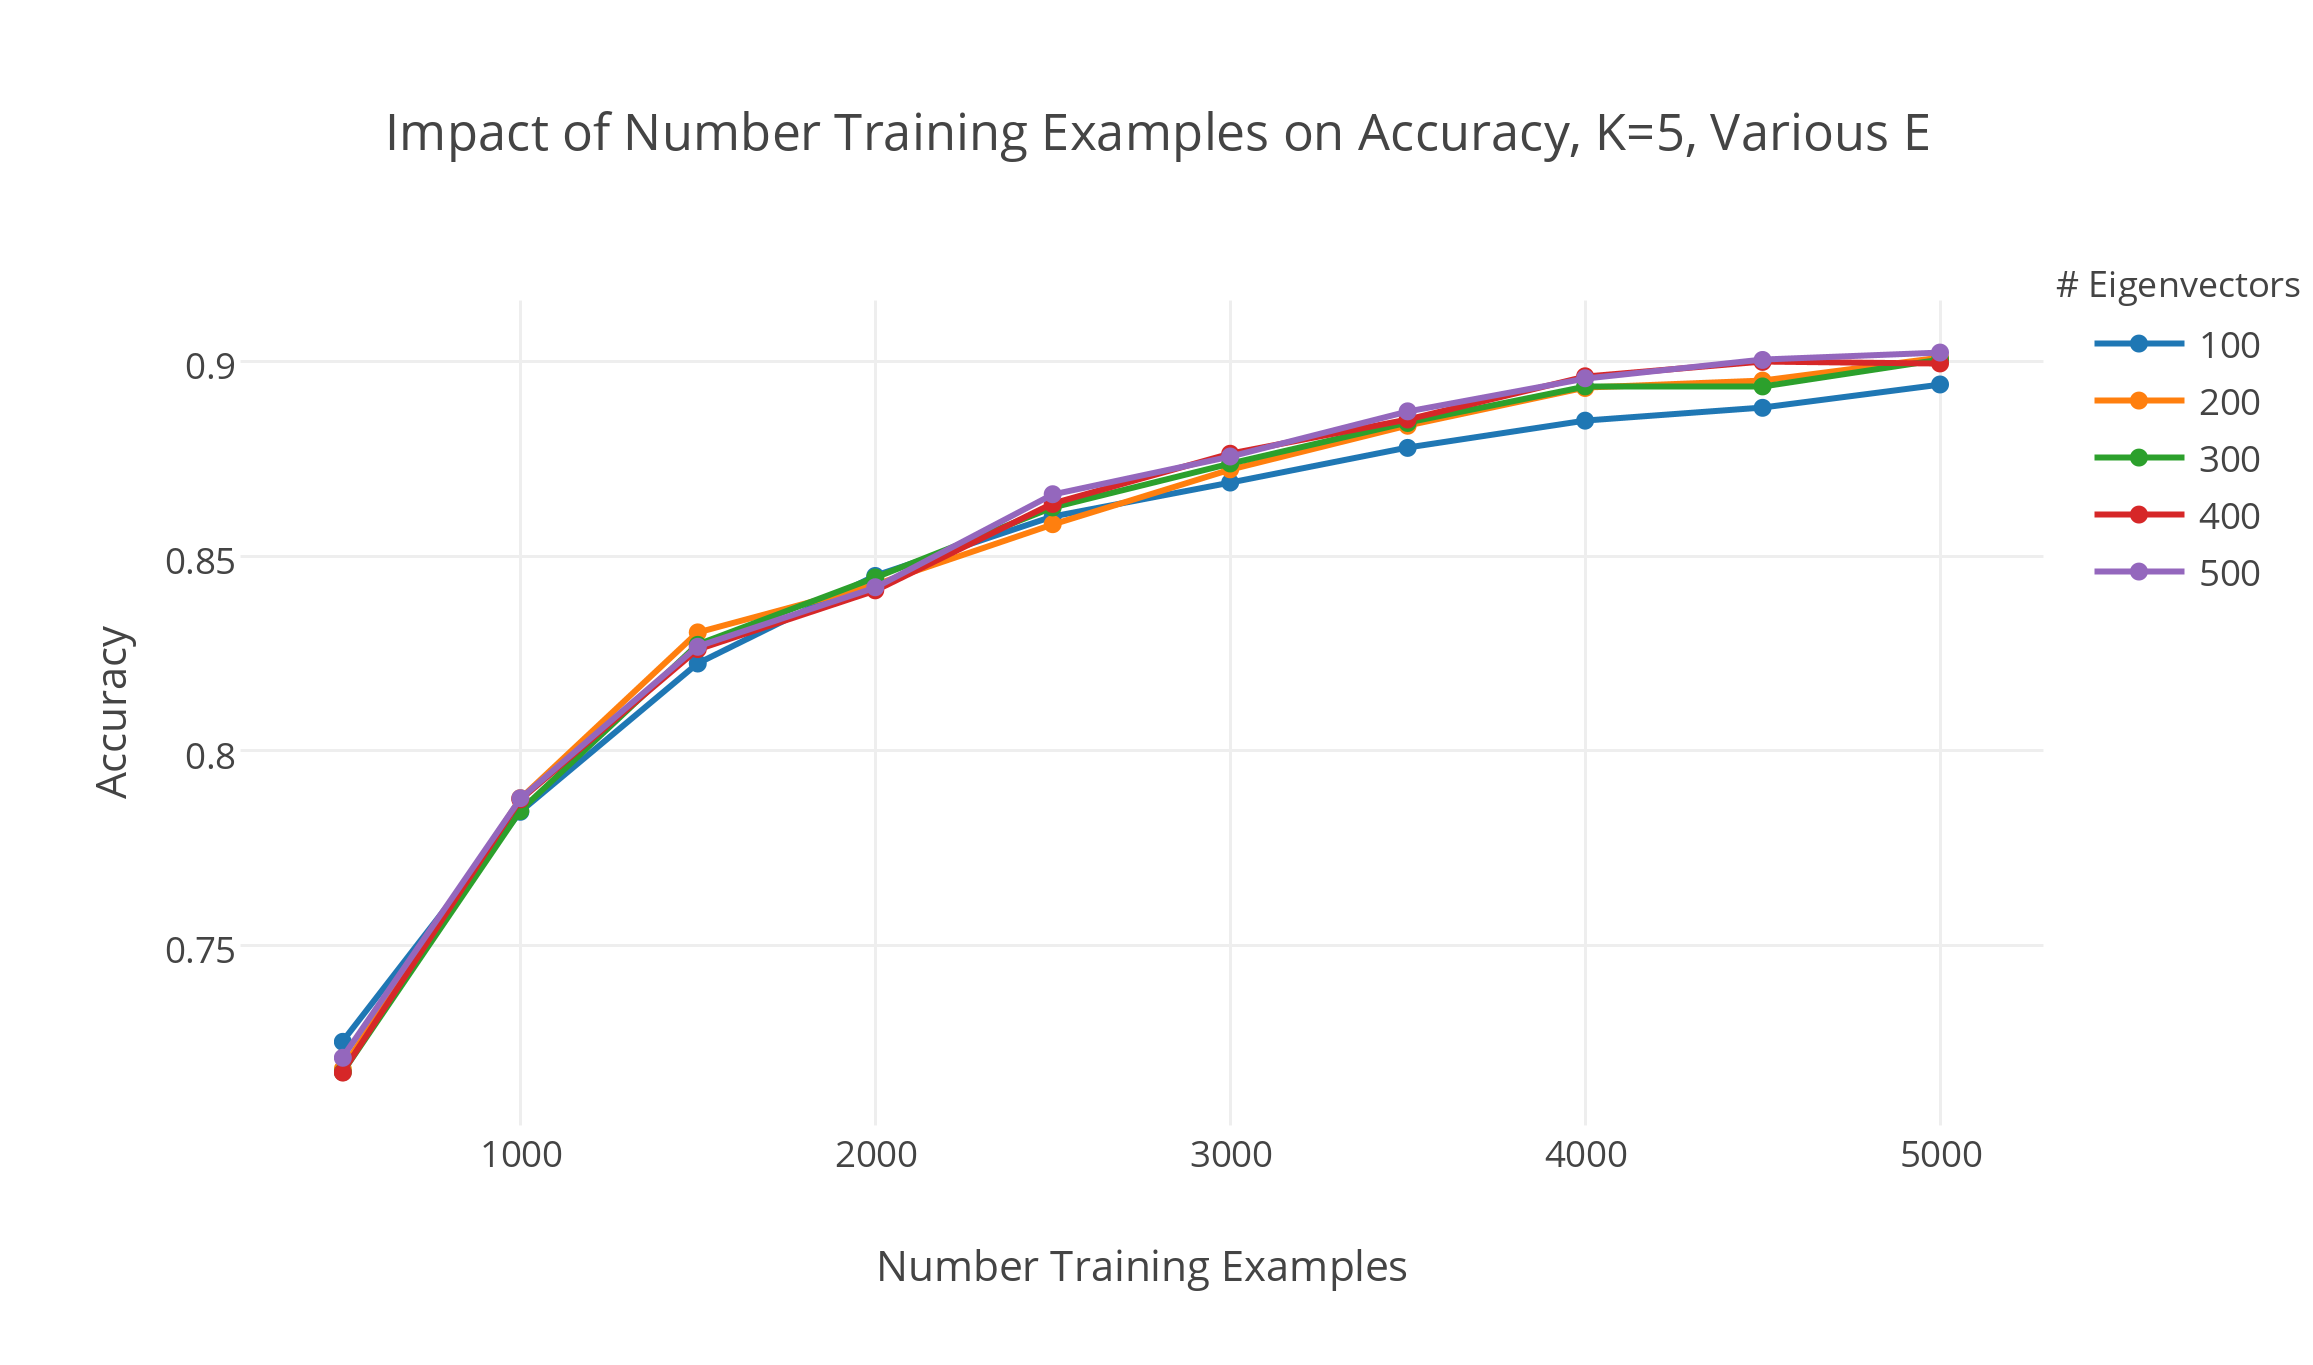
\includegraphics[width=80mm]{impact_of_number_training_examples_on_accuracy2c_k52c_various_e.png}%
            \label{fig:right}%
        }\hfill%
        \subfloat[K=7 and various E]{%
        	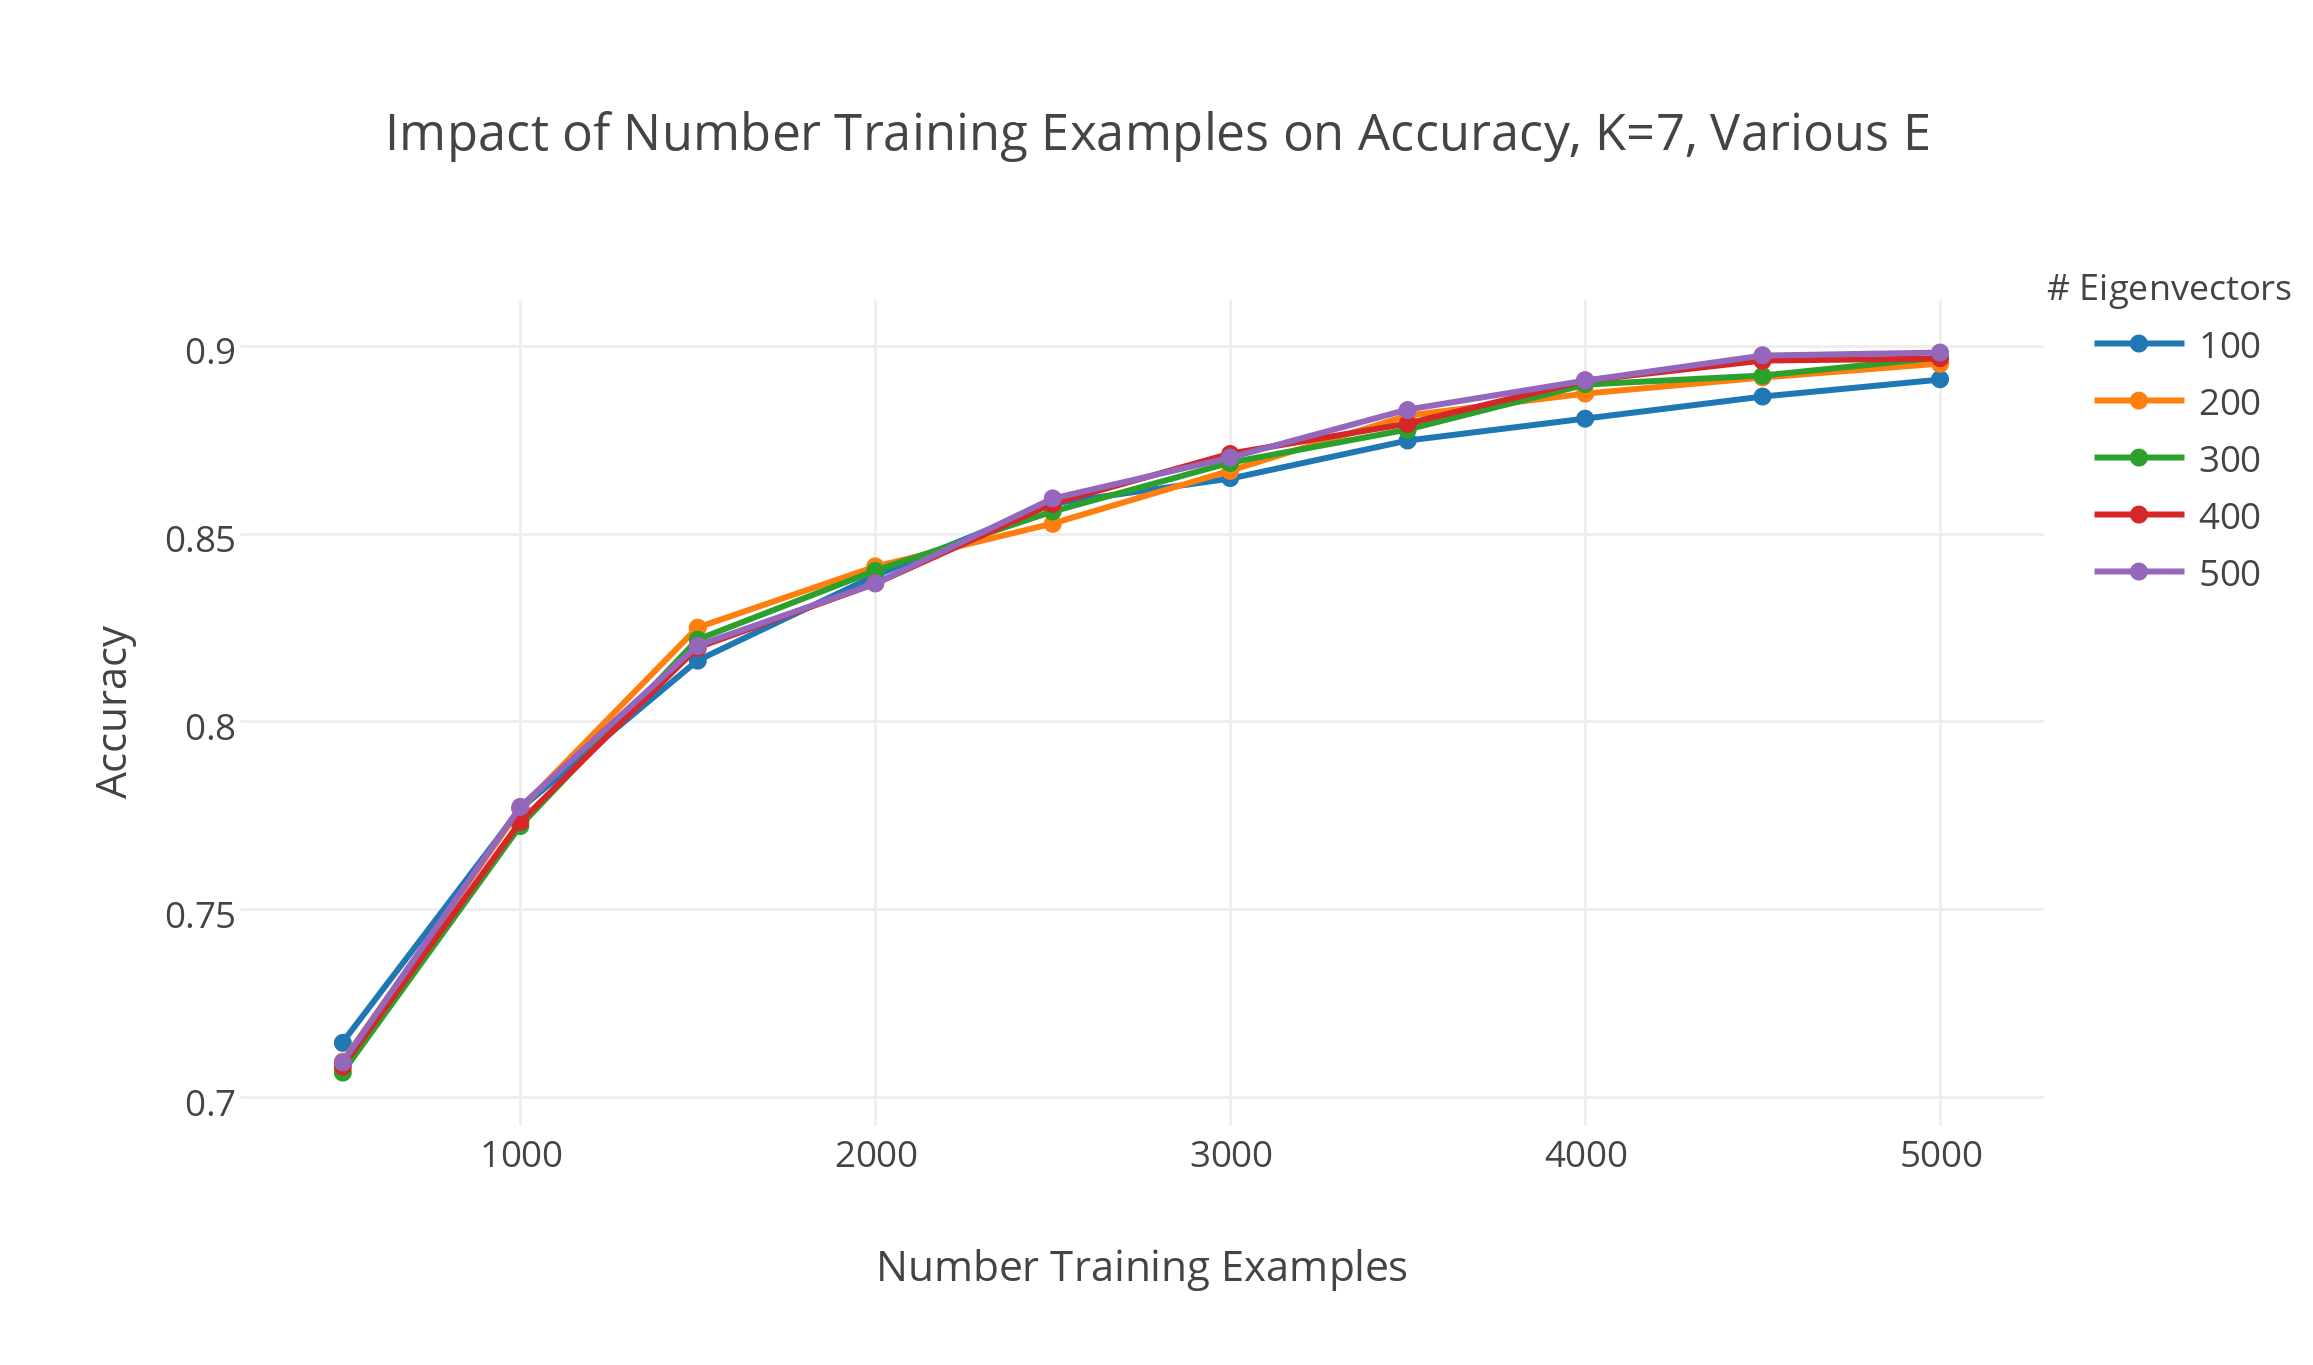
\includegraphics[width=80mm]{impact_of_number_training_examples_on_accuracy2c_k72c_various_e.png}%
            \label{fig:right}%
        }
    \caption{\textit{The impact of the number of training examples on overall classification accuracy, with various K and various E.}}
    \label{fig:default}
\end{figure}  

Based on Figure 2, adding training examples provided a significant benefit initially when there was a small set of training examples used while the effect of increasing the training set size gradually decreases as the current training set size increases (e.g. the accuracy increase between \(T=500\) to \(T=1000\) is greater than \(T=3500\) to \(T=4000\)). The clumping behavior of the different lines for the number of top eigenvector values used in each plot is explained in section 3.2.2.

With enough training examples and parameter tuning, I was able to go past 90\% accuracy in the classification step or come close to it within 0.01\%. Table 1 shows some of the configurations in which I achieved an accuracy greater than 90\%. 

\begin{table}[H]
\centering
\begin{tabular}{c|c|c|c}
T & E & K & Accuracy (in \%) \\\hline
10000 & 500 & 7 & 91.91 \\
10000 & 300 & 7 & 91.74 \\
7500 & 500 & 5 & 91.13 \\
4500 & 500 & 5 & 90.94 \\
\end{tabular}
\caption{\label{tab:widgets} A small selection of configurations that provided accuracy over 90\%.}
\end{table}

In addition to the fact that the classifier can be tuned to classify with an accuracy greater than 90\%, the results in the table suggests that throwing more training data at the classifier will continue to plateau without further intrinsic tuning. The decreasing shape of curvature of the lines in Figure 2 also supports evidence to this notion. While adding more training data helped initially, to further improve the classifier quicker I will likely need to consider more options such as tuning the intrinsics of k-Nearest Neighbors classifier (e.g. weighting samples in the neighborhood, experimenting with other different distance metrics), utilizing a different set of training data providing more dissimilar examples or leveraging more/better features.

\subsection{Varying Number of Selected Eigenvectors}

\subsubsection{Setup}

I reused the data generated from section 3.1.1 and I ran the overall eigenvector retrieval and classification procedure for each \(\left\{ T,E,K \right\}\) combination, where \(T = 2500\}\), \(E \in \{10, 50, 100, 250, 500\}\), and \(K \in \{1,3,5,7\}\) for further granularity. 

\subsubsection{Results and Observations}

Figure 3 utilizes the data described in section 3.1.1 and describes the slice of the data where \(T=2500\) and \(K=3\). 

\begin{figure}[h]%
	\centering
    	\subfloat{%
        	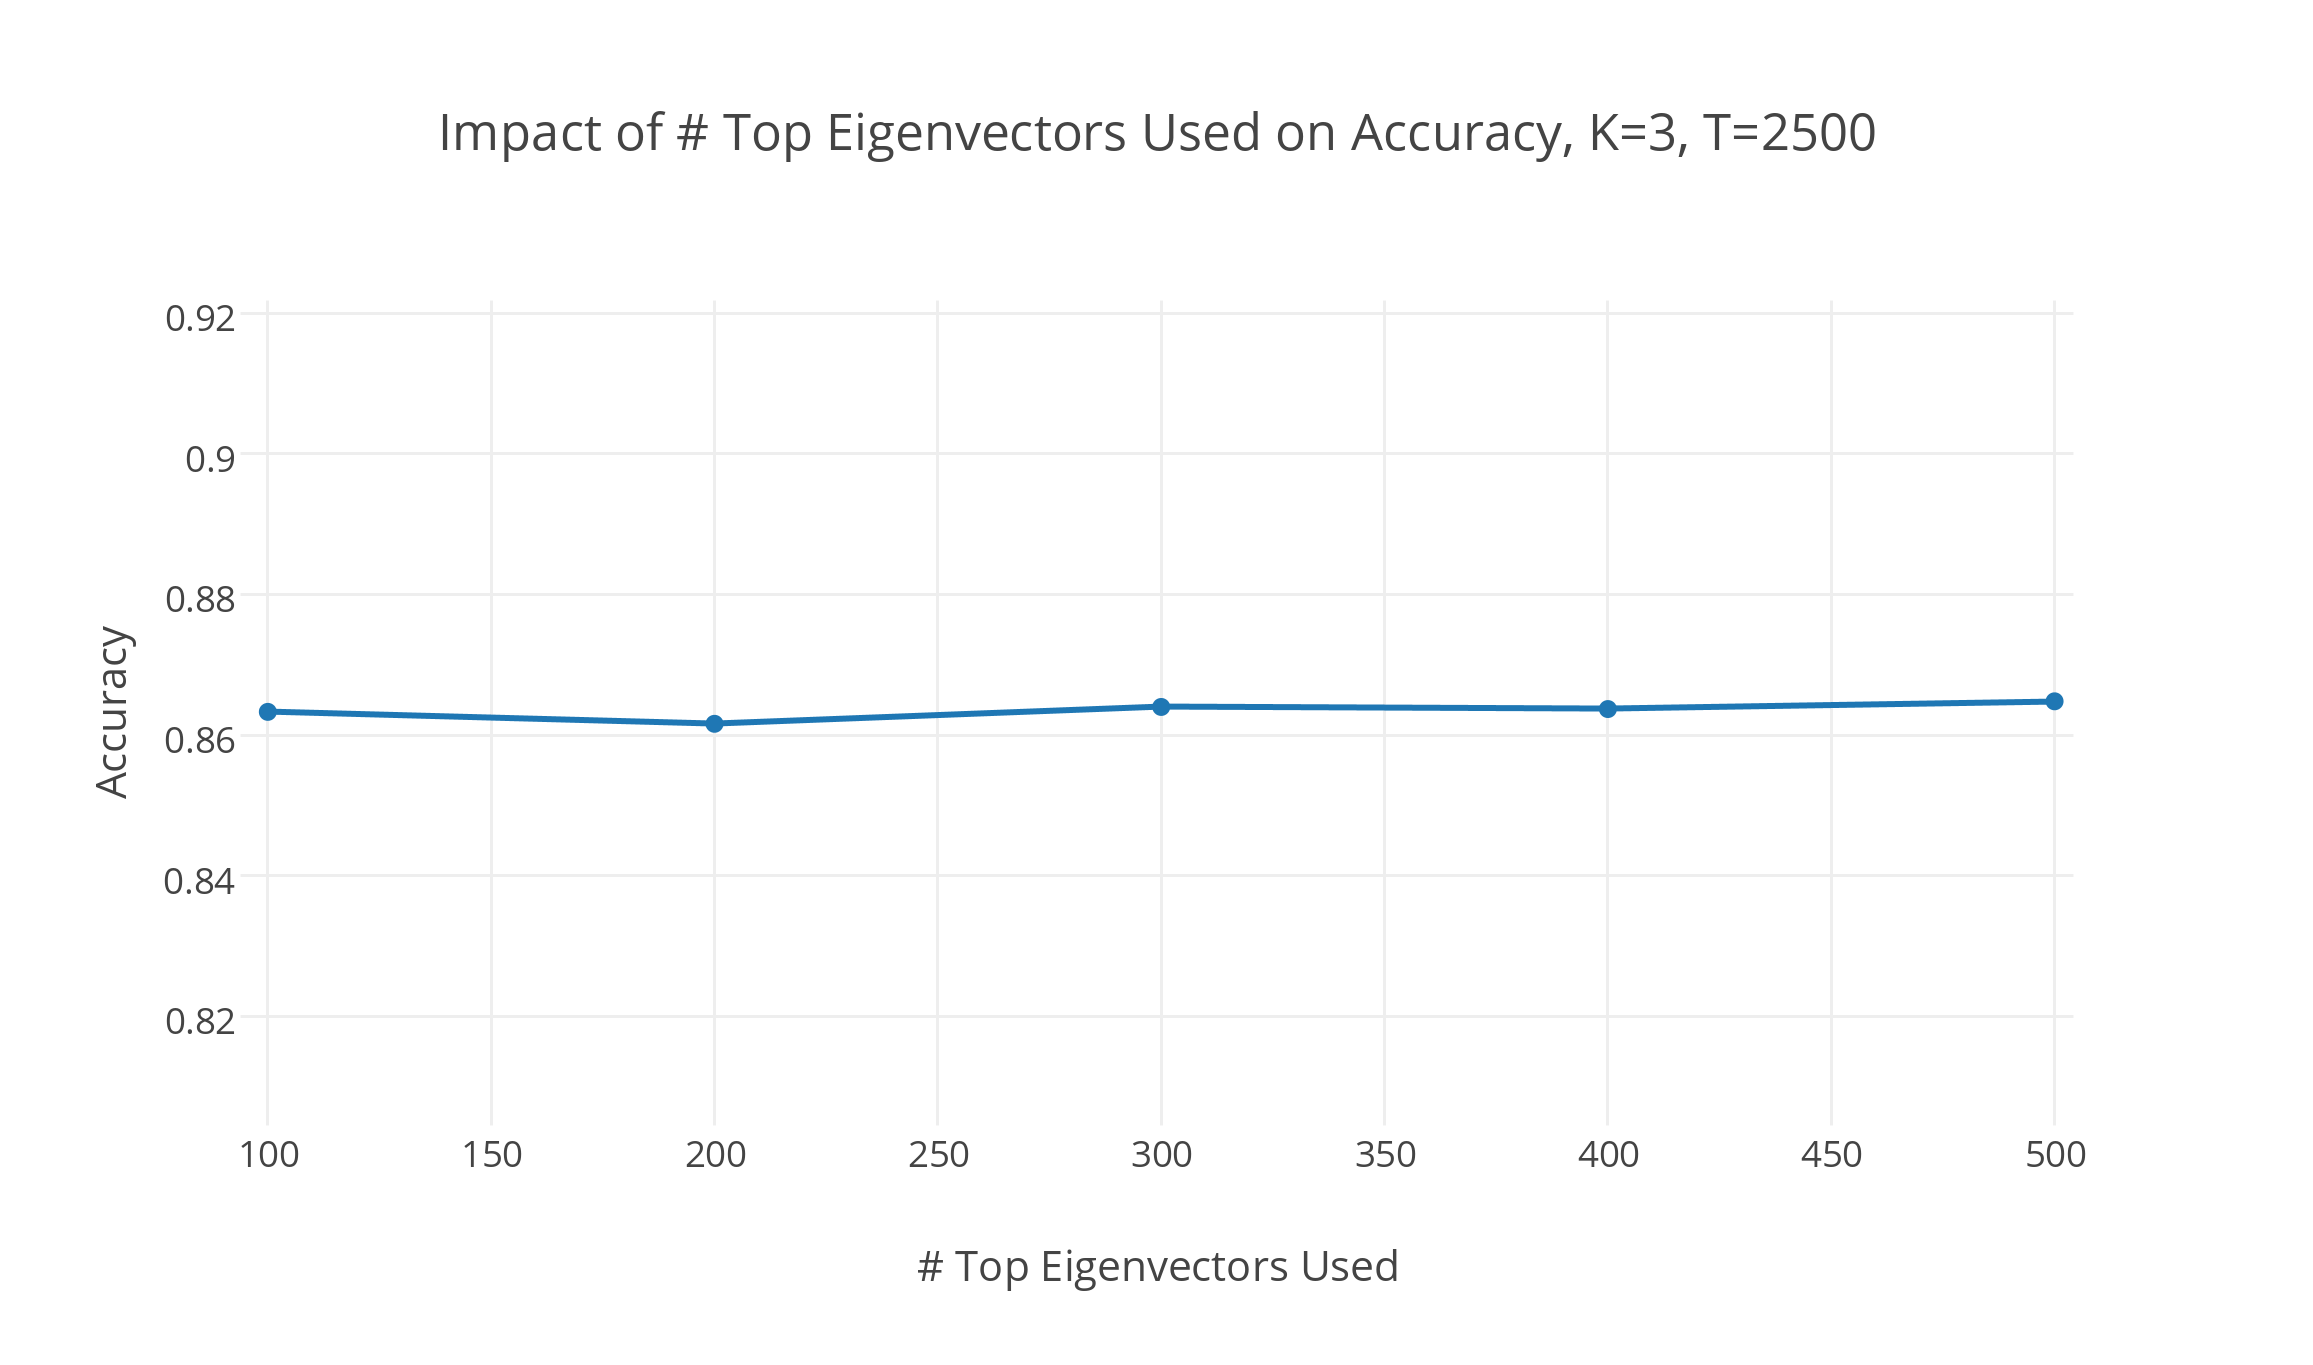
\includegraphics[width=100mm]{eigenvectors_used_slice.png}%
        }\hfill%
    \caption{\textit{Impact of Top Eigenvectors chosen on Accuracy at K=3 and T=2500}}
    \label{fig:default}
\end{figure}

In Figure 3, despite varying the values of \(E\) between \(100-500\), there is but a slight change in the overall accuracy. This observation implies that there is little difference in accuracy gain in selecting either the top 100 or top 500 eigenvectors for projection into a reduced eigenspace (i.e. the change was less than 0.005). In other words, for these values of \(K\) and \(T\), the 400 features after the first top 100 eigenvectors provided little more information. As a result, the result helps further establish the potential of dimensionality reduction by the use of Principal Component Analysis. Given that the first 100 features were the highest impacting components, the results suggest that we don't receive significantly more information or performance by including the rest of the components. This highlights that the usage of Principal Component Analysis allows for the use of smaller matrices in order to achieve efficiency gains.

Figure 4 describes the data mentioned in the setup of this section (i.e. Section 3.2.2), generated in order to view where the gain in accuracy begins to plateau for increases in values of \(E\).

\begin{figure}[h]%
	\centering
    	\subfloat{%
        	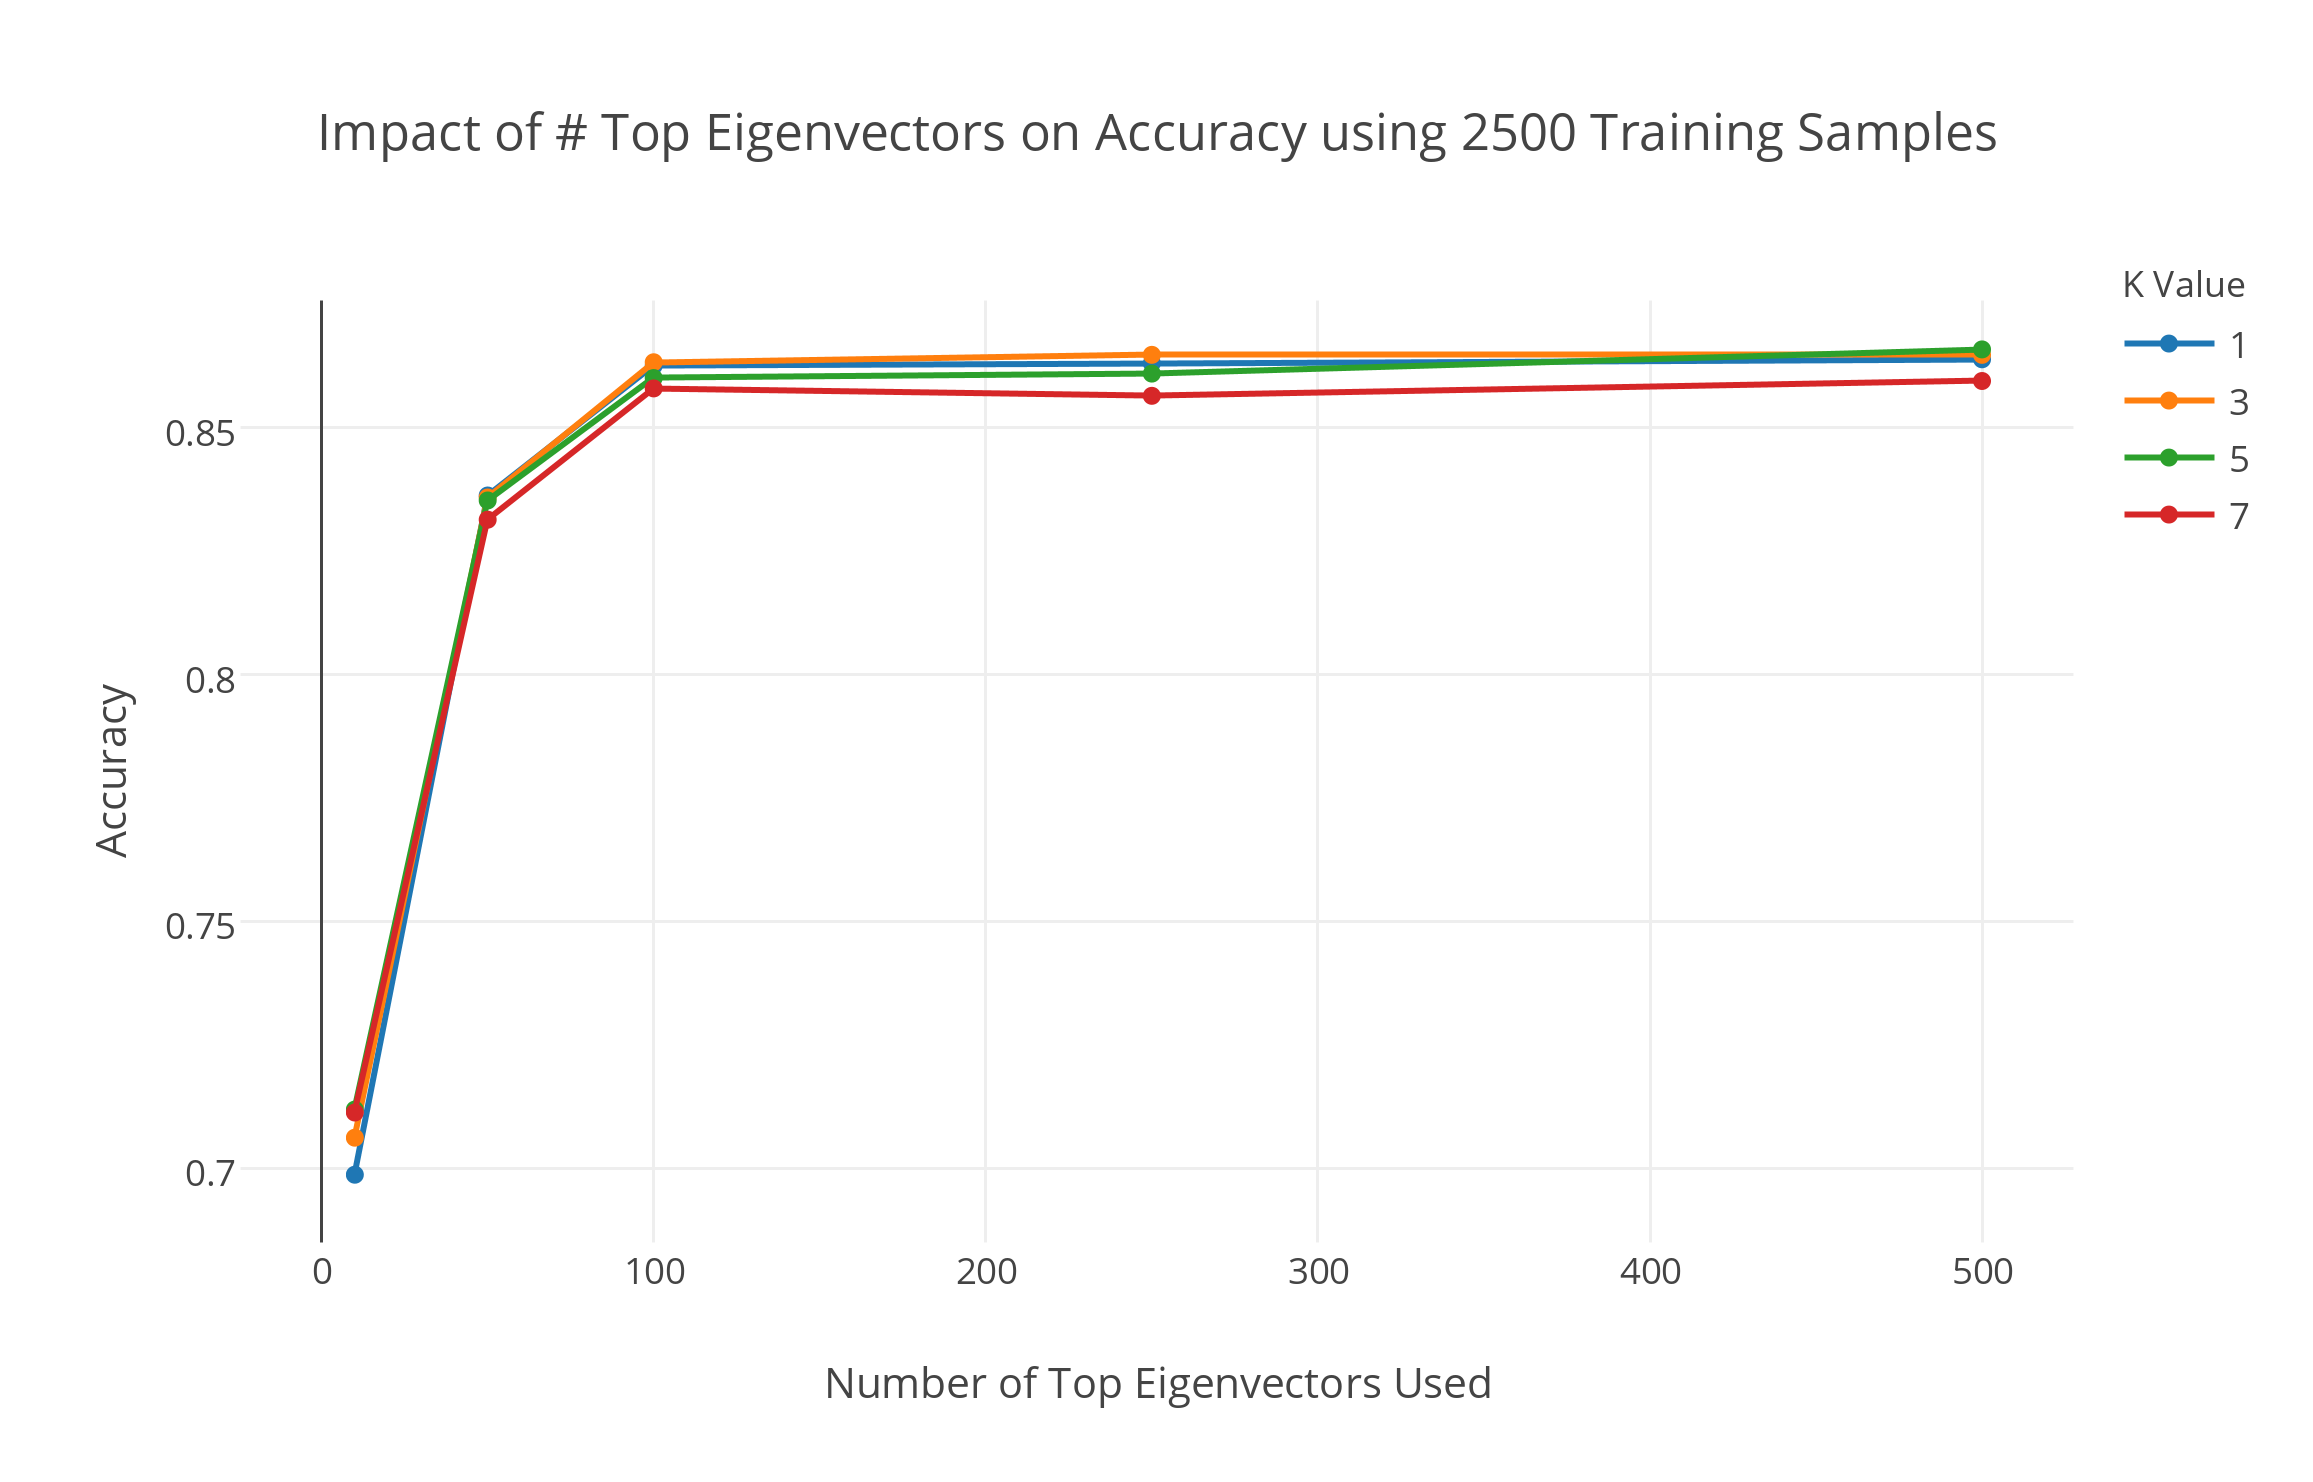
\includegraphics[width=100mm]{eigenvector_number_impact.png}%
        }\hfill%
    \caption{\textit{Impact of Top Eigenvectors chosen on Accuracy at various K and T=2500}}
    \label{fig:default}
\end{figure}

The graph shows that, for the case of \(T=2500\) and varying values of K, the accuracy essentially plateaus quite early. Based on the graph, the largest gain occurred due to the first 50 top eigenvectors. This further reinforces the notion that, in a set of eigenvectors of the data's covariance matrix sorted descending by their corresponding eigenvalue, a particular selection of the top eigenvectors can help represent a very good approximation of the overall variance in the data set.

\subsection{Varying k-Nearest Neighbor}

\subsubsection{Setup}

The data generated for the experiments above, as described in Sections 3.1.1 and 3.2.2, was reused to analyze the effects of different values of K for the k-Nearest Neighbors classifier. The values for which K was tested were all chosen specifically to be odd numbers to avoid any potential ties.

\subsubsection{Results and Observations}

In general, the optimal K value for the K-Nearest Neighbors resided in the lower numbers, generally around 5. However, much larger values resulted in a gradual decrease in accuracy. This is captured in Figure 5 and Figure 6.

\begin{figure}[h]%
	\centering
    	\subfloat{%
        	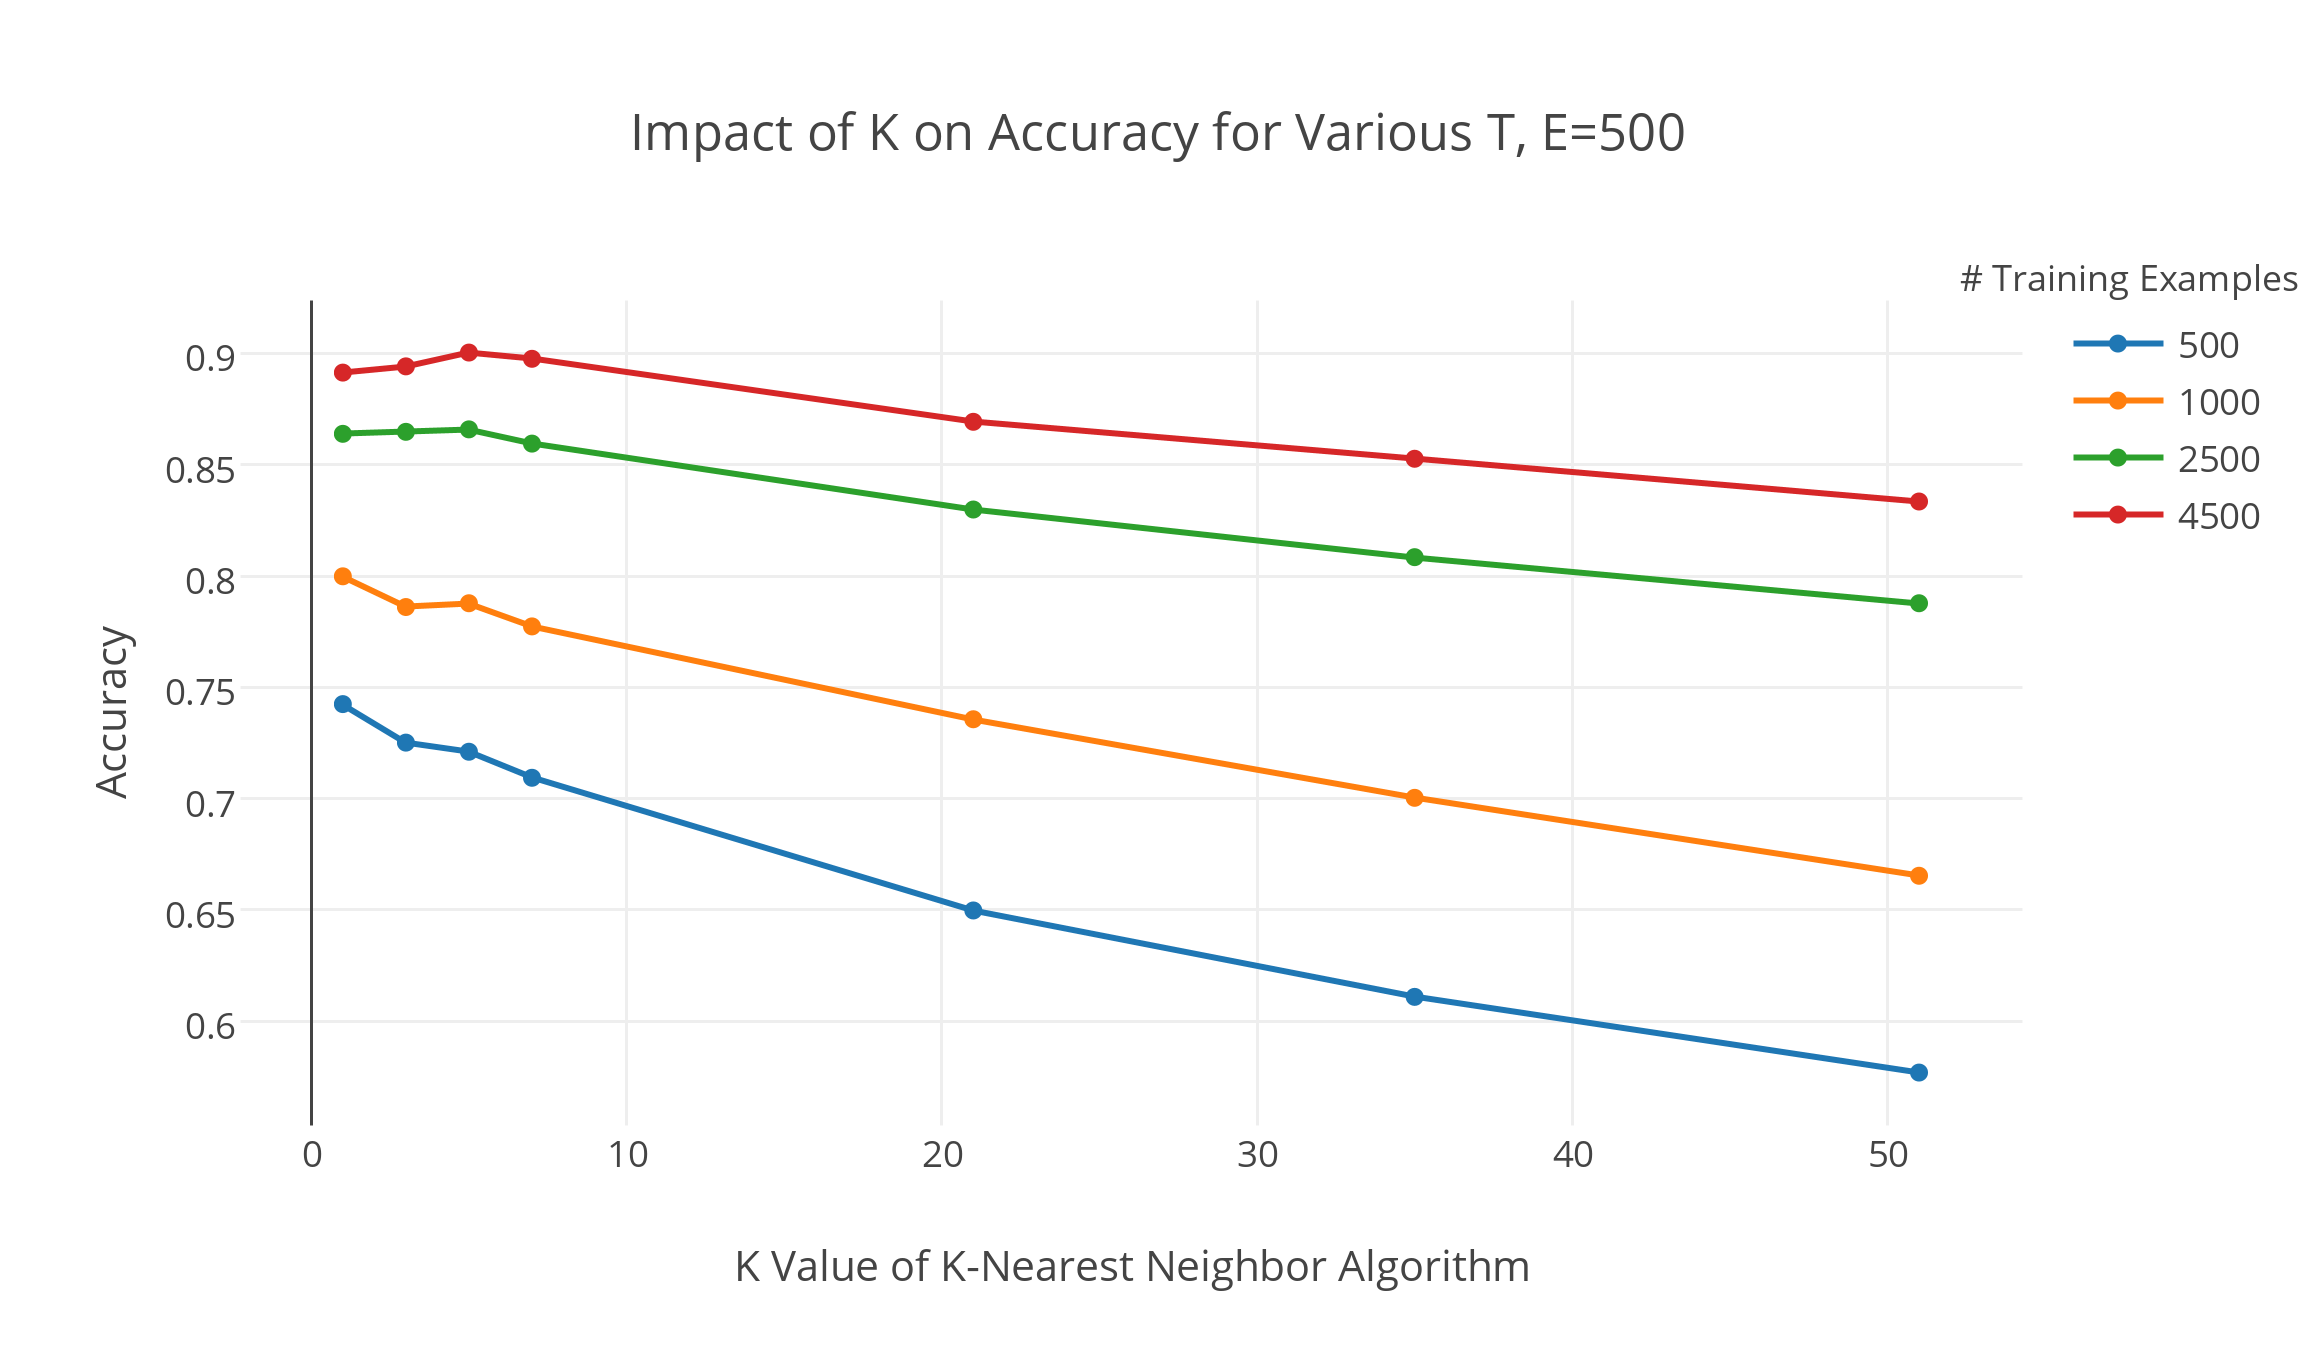
\includegraphics[width=100mm]{impact_of_k_on_accuracy_for_various_t2c_e500__3_.png}%
        }\hfill%
    \caption{\textit{Impact of K at various T and E=500}}
    \label{fig:default}
\end{figure}

Relatively, the optimal K was larger for runs with larger training image set size. Intuitively, the result makes sense. With smaller training image set sizes, there is a larger likelihood for a larger impact of and presence of noise and overfitting. This behavior is further captured in Figure 6.

\begin{figure}[h]%
	\centering
    	\subfloat[T=50,E=50]{%
        	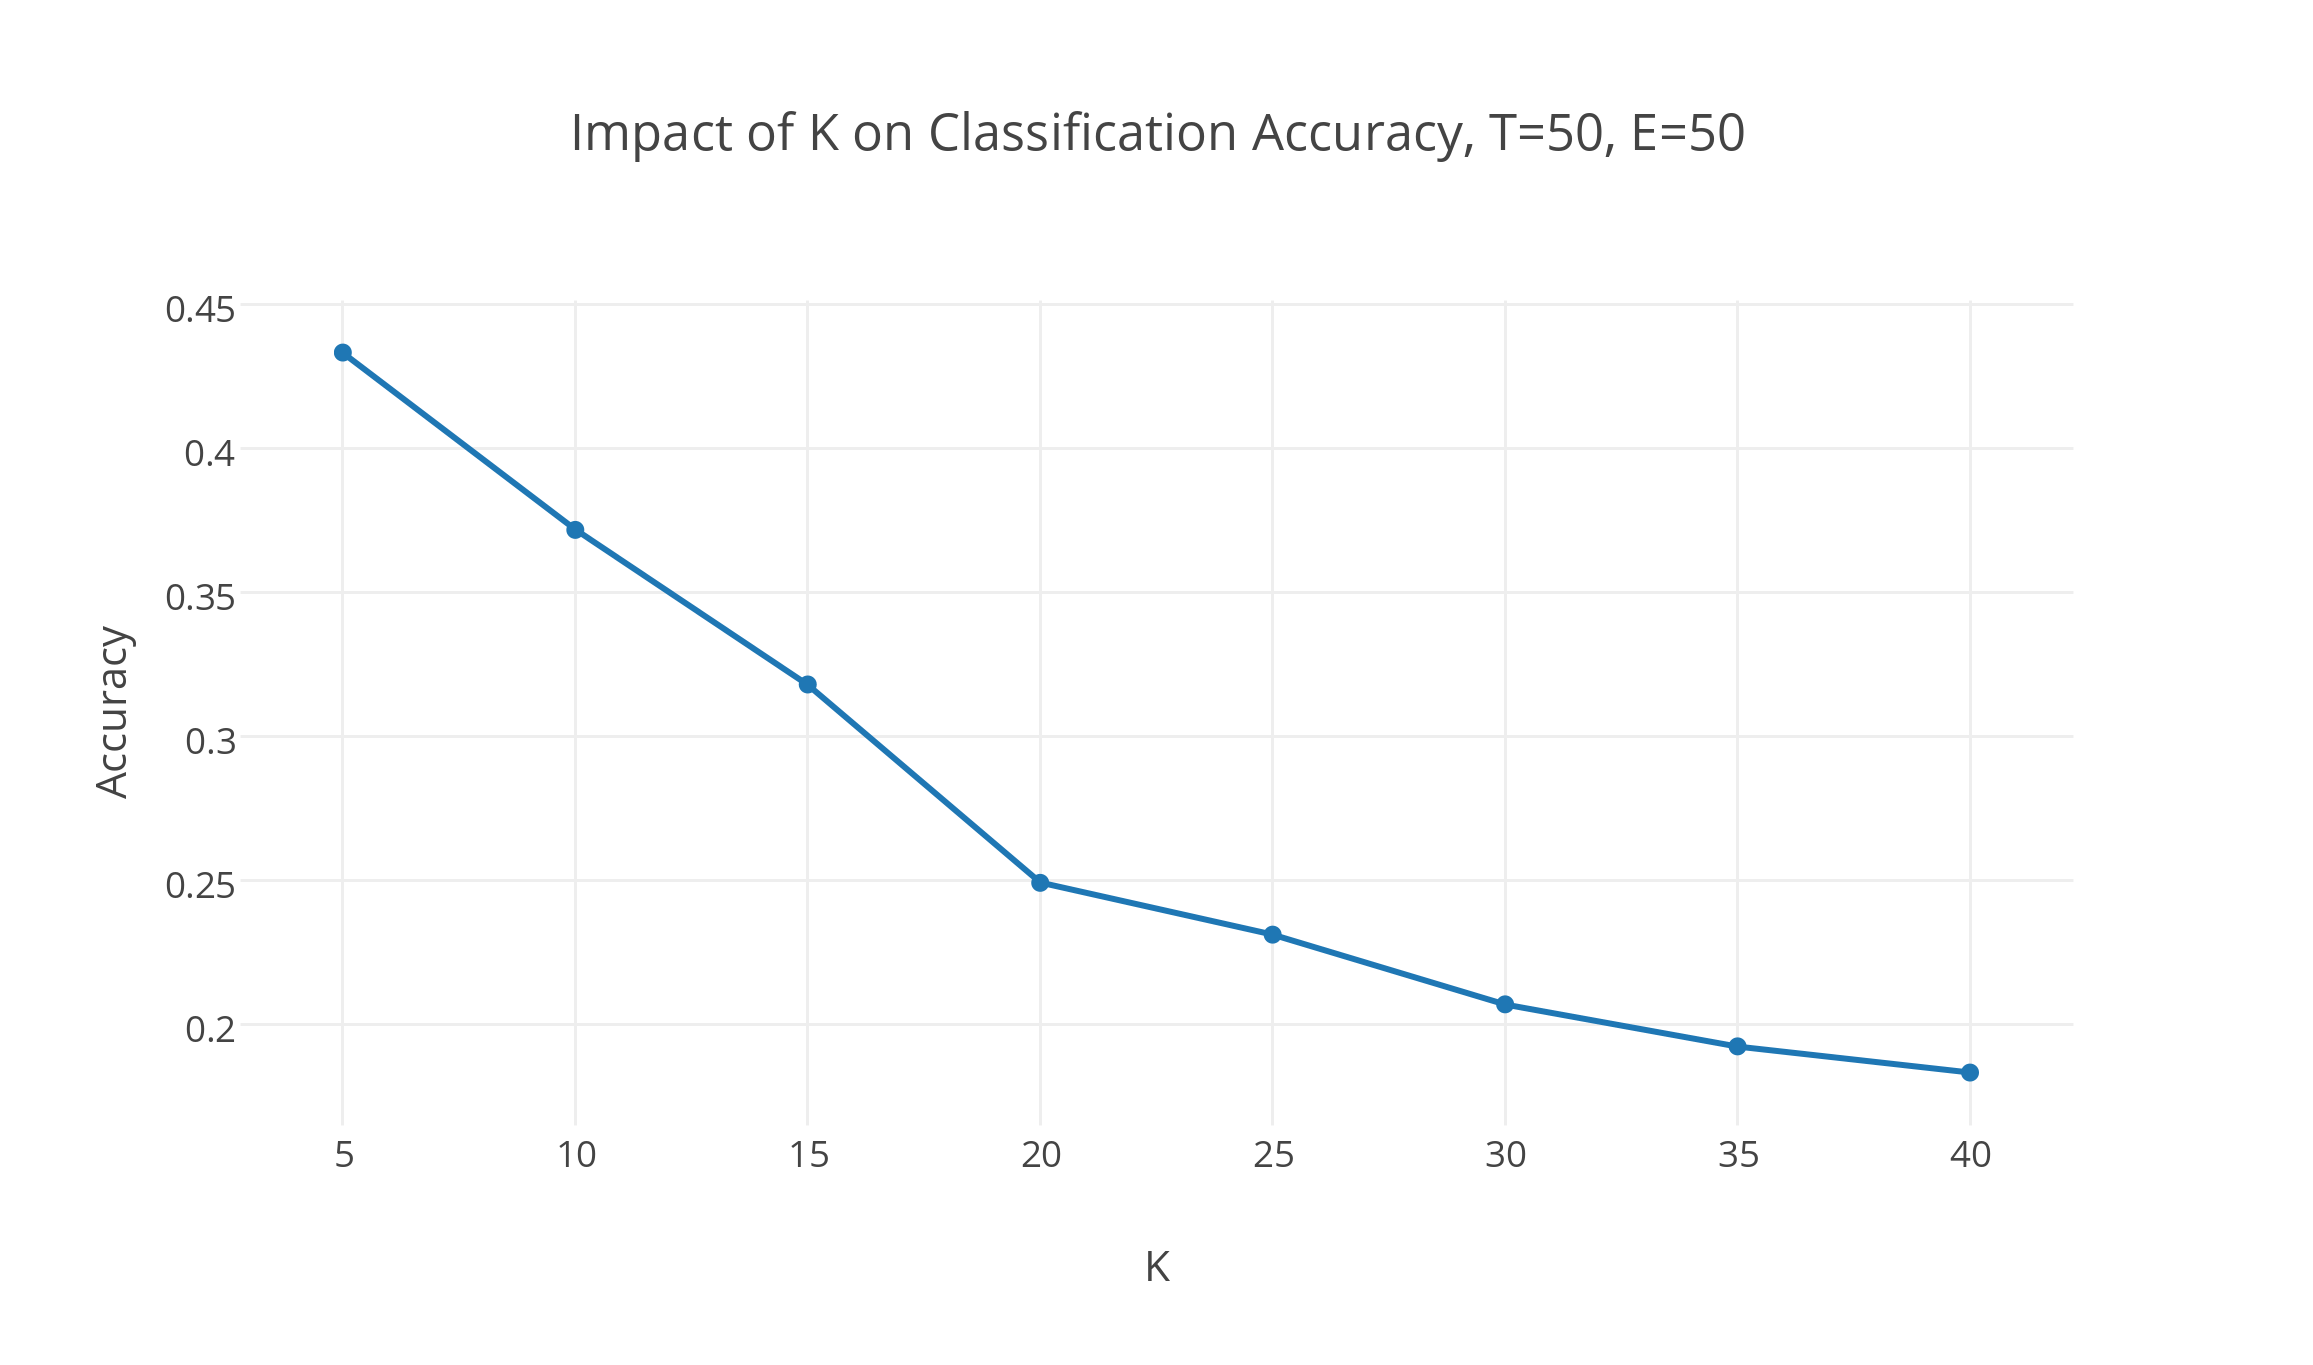
\includegraphics[width=50mm]{impact_of_k_on_classification_accuracy2c_t502c_e50.png}%
            \label{fig:left}%
        }\hfill%
        \subfloat[T=50,E=10]{%
        	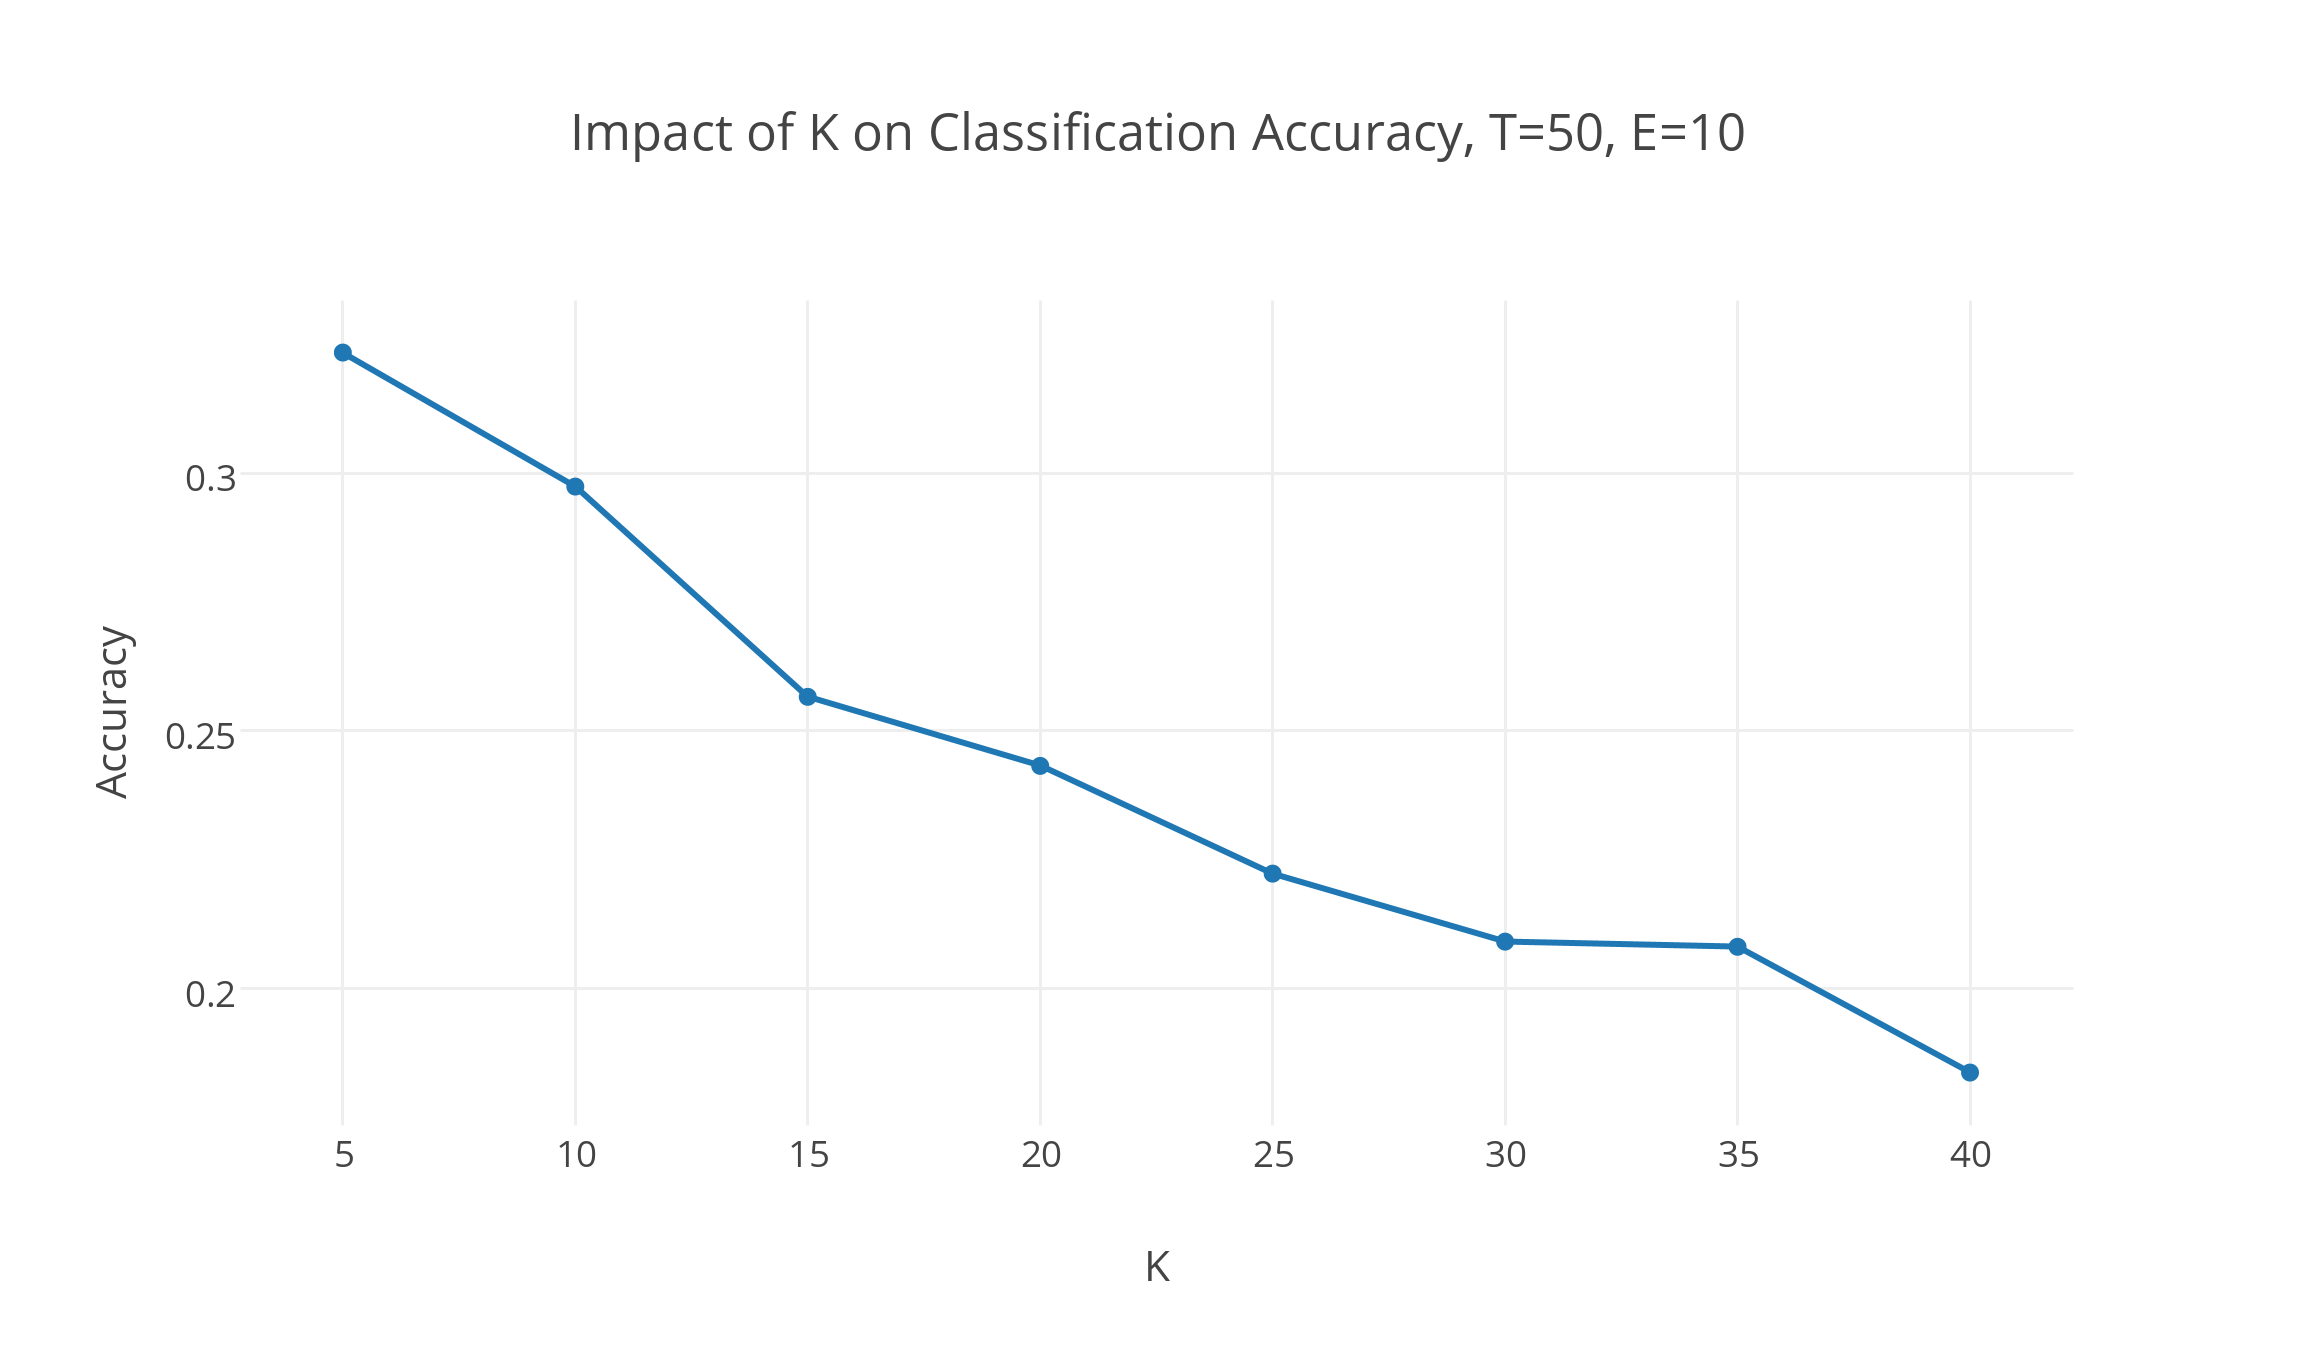
\includegraphics[width=50mm]{impact_of_k_on_classification_accuracy2c_t502c_e10.png}%
            \label{fig:center}%
        }\hfill%
		\subfloat[T=100,E=10]{%
        	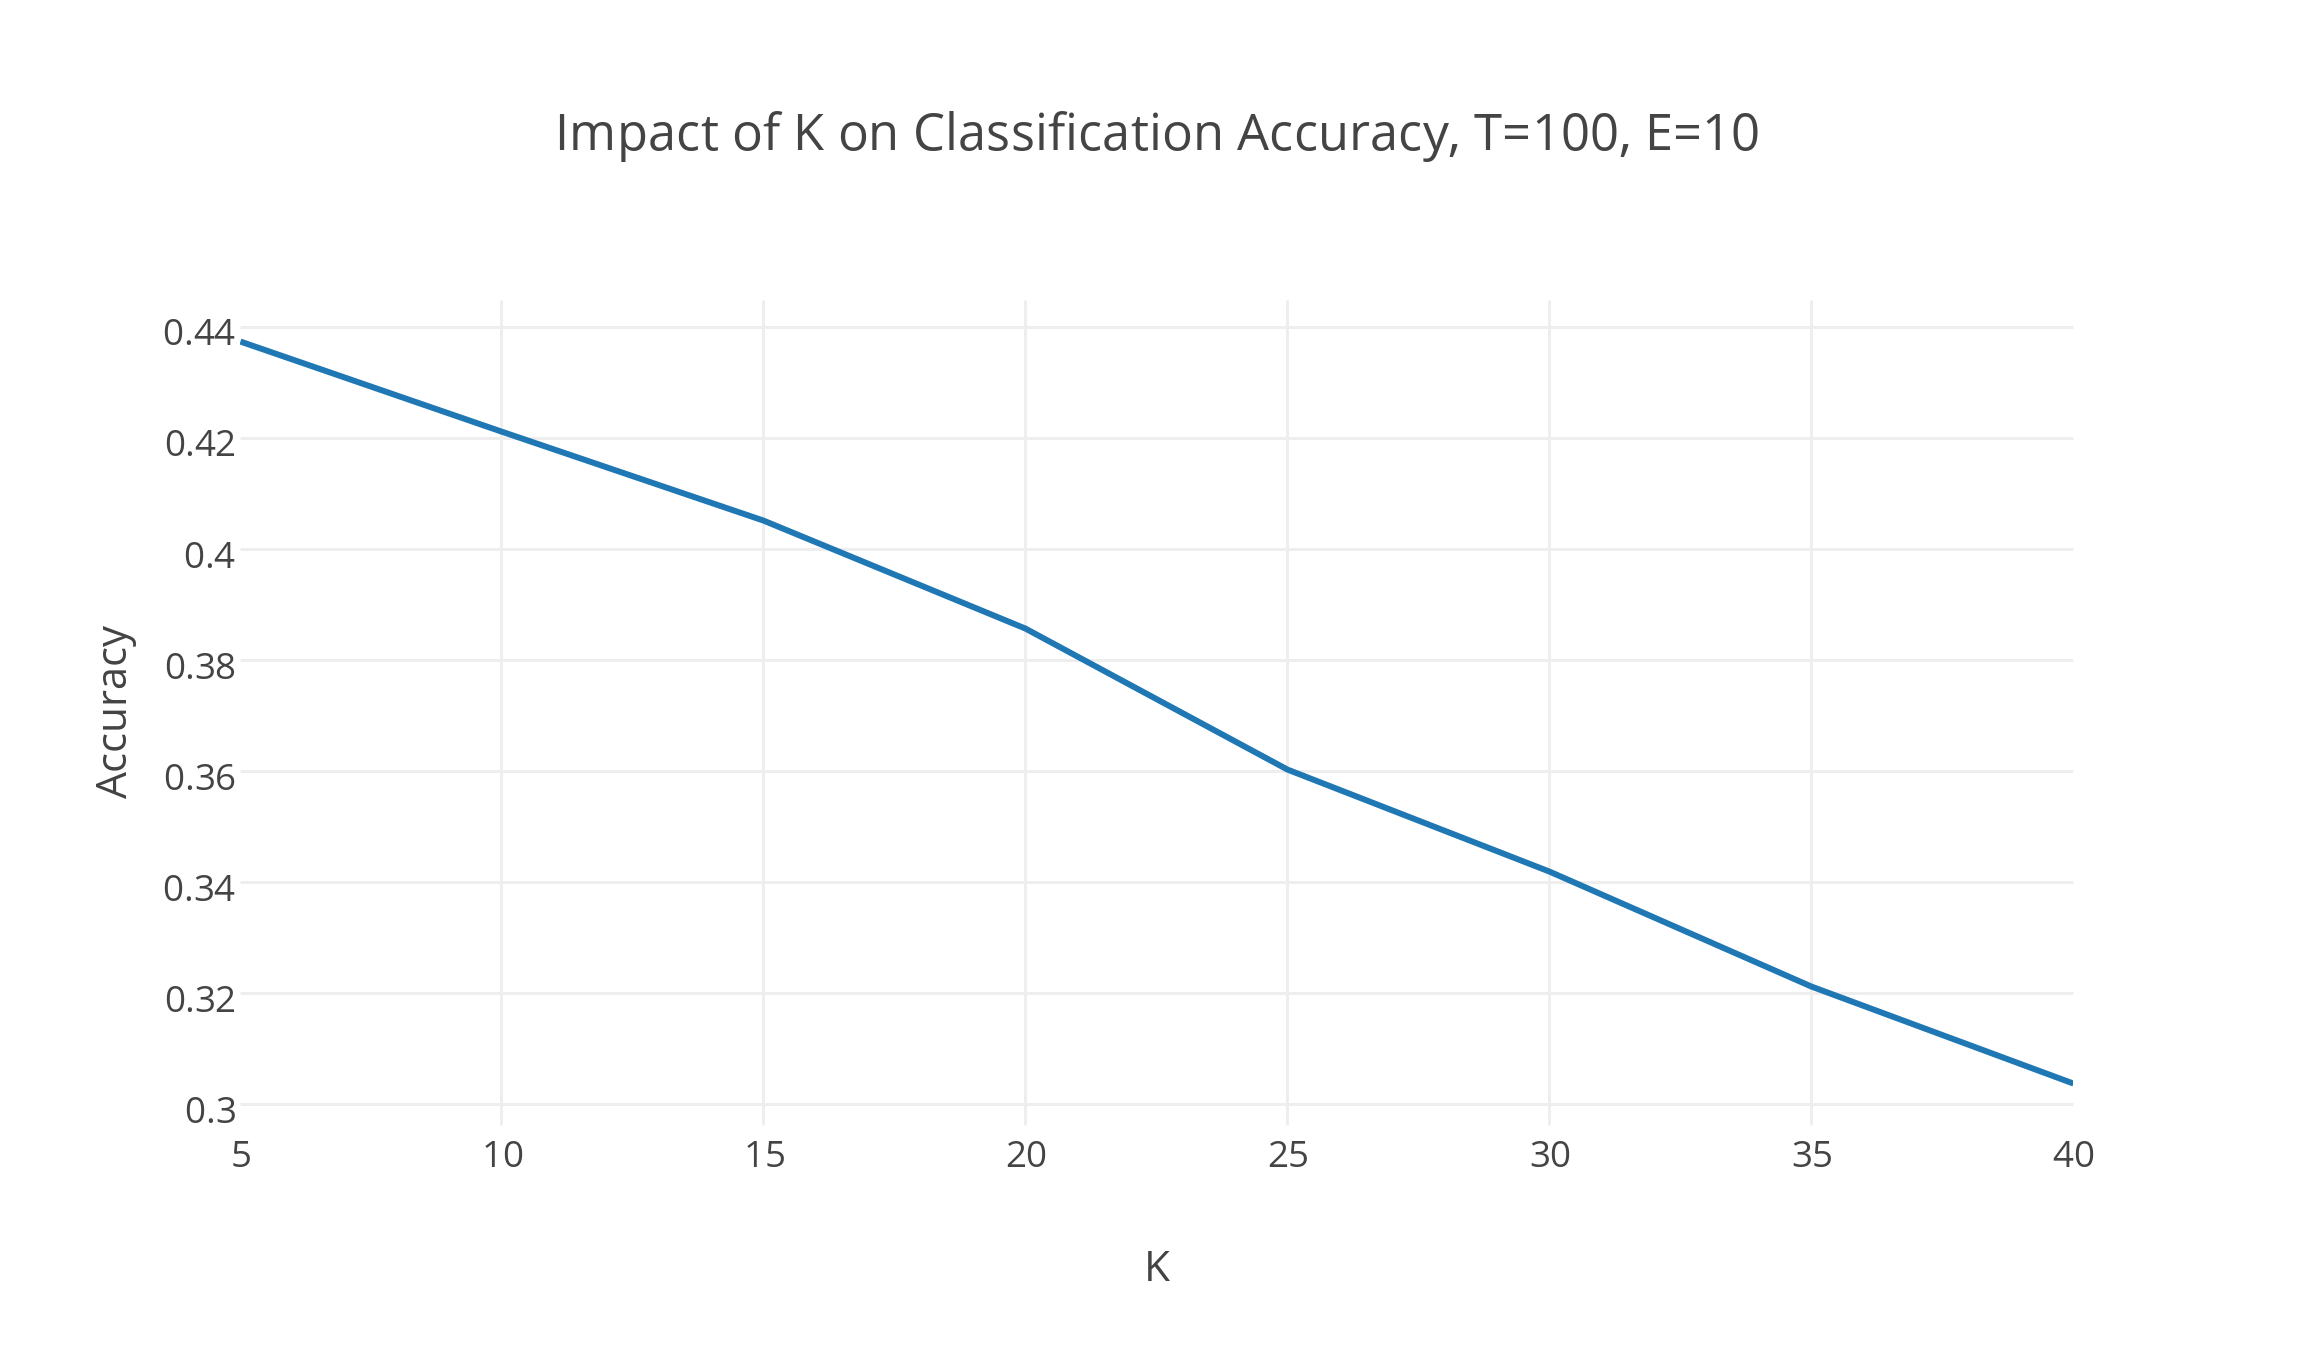
\includegraphics[width=50mm]{impact_of_k_on_classification_accuracy2c_t1002c_e10.png}%
            \label{fig:right}%
        }
    \caption{\textit{Impact of values of K on classification accuracy for various T,E values.}}
    \label{fig:default}
\end{figure}

For various small values of the training set size, Figure 6 displays the overall accuracy against changing values of K. The fact that the overall accuracy is quite low and peaks at \(K=1\) indicates the the model created in training doesn't truly fit the overall data well. In comparison, it can be noted that as the size of the training set increased in the experiments, larger neighborhoods were able to be developed. 

\section{Concluding Notes}

I was surprised to find a high degree of accuracy with the seemingly simplistic approach that we took to classify digits. The experiments made the advantages of Principal Component Analysis clear. Essentially, Principal Component Analysis, as the name suggests, allows for the focus on the principal components that cause the most variation rather than everything, providing the opportunity for large gains in efficiency through dimensionality reduction.

However, I am interested in expanding the building and testing of the classifier in this assignment. For example, how would this classifier operate on other test sets and in generic cases? In addition, based on the approach to finding eigendigits, the assignment essentially leveraged each pixel of each input image as a feature. The inclusion of other more/better features such as particular curvature or edges may be an interesting extension to this assignment for future work.

\end{document}